\graphicspath{{chapters/deep_learning/}}


\chapter{Deep CCA and CCA for Self-Supervised Learning}\label{chap:deep_learning}
\minitoc
% chktex-file 44
% chktex-file 3
\section*{Preface}

This chapter is based on work presented in \citet{chapman2023cca} and \citet{chapman2023efficient}.

\section{Introduction}

Deep CCA \citep{andrew2013deep} secured a runner-up position for the test-of-time award at ICML 2023 \citep{ICML2023TOT}.
However, its direct application has been limited in large datasets due to biased gradients in the stochastic minibatch setting.
There have since been proposals to scale-up Deep CCA in the stochastic case with adaptive whitening \cite{wang2015stochastic} and regularization \cite{chang2018scalable}, but these techniques are highly sensitive to hyperparameter tuning.

Self-Supervised Learning (SSL) methods have reached the state-of-the-art in tasks such as image classification \citep{balestriero2023cookbook}, learning representations without labels that can be used to classify images using a linear probe in the zero-shot setting.
Recently, a family of SSL methods that are closely aligned with Canonical Correlation Analysis (CCA) has garnered interest.
This family notably includes Barlow Twins \citep{zbontar2021barlow}, VICReg \citep{bardes2021vicreg}, and W-MSE \citep{ermolov2021whitening} and they aim to transform a pair of data views into similar representations, similar to the objective of CCA. Similarly, some generative approaches to SSL\cite{sansone2022gedi} bear a striking resemblance to Probabilistic CCA\cite{bach2005probabilistic}.
These connections have started to be explored in \cite{balestriero2022contrastive}.

In this chapter, we propose a novel formulation of Deep CCA that is unbiased in the stochastic setting and scales to large datasets.
We also propose a novel SSL method, SSL-EY, that is competitive with existing methods on CIFAR-10 and CIFAR-100.
We highlight the connections between our work and existing SSL methods, and show that our method is more robust to hyperparameter tuning.

\section{Background}

\subsection{Deep Learning}

Deep learning is a subfield of machine learning that uses functions parameterised by neural networks.
Deep learning has been applied to a wide range of domains, including computer vision, speech recognition, natural language processing, and bioinformatics, where they have produced state-of-the-art results on many tasks.
Neural networks are usually composed of many linear layers followed by nonlinear activation functions such as the rectified linear unit (ReLU).
The ReLU activation function is defined as $\ReLU(x) = \max(0, x)$.
The ReLU activation function is piecewise linear, and so the composition of ReLU activations with linear functions is a piecewise linear function.
It has been shown that neural networks with ReLU activations can approximate any continuous function on a compact set to arbitrary accuracy \citep{perekrestenko2018universal}, and so are universal function approximators.
This flexibility, combined with increasingly large datasets, allows neural networks to learn complex functions from data.
Owing to the size of the models and datasets, neural networks are usually trained using the backpropagation algorithm and stochastic gradient descent (SGD) \citep{amari1993backpropagation}.



\subsection{DCCA and Deep Multiview CCA}

Thus far, our focus has been on linear Canonical Correlation Analysis (CCA). However, in dealing with high-dimensional and complex data structures commonly found in modern applications, nonlinear extensions of CCA become essential. Deep CCA (DCCA) and Deep Multiview CCA (DMCCA) represent such nonlinear extensions, aiming to capture more intricate relationships between data views.

In essence, the objective of DCCA and DMCCA is to learn nonlinear representations of data that are linearly correlated across different views. We define this goal using our $\MCCA$ notation:
\begin{align}
    \label{eq:DMCCA-def}
    \norm{\MCCA_K\left(Z^{(1)}, \ldots, Z^{(I)}\right)}_2
\end{align}
where $Z^{(i)} = f^{(i)}(X^{(i)}; \theta^{(i)})$ are representations learned by neural networks for each view $i \in [I]$.

\begin{figure}
    \centering
    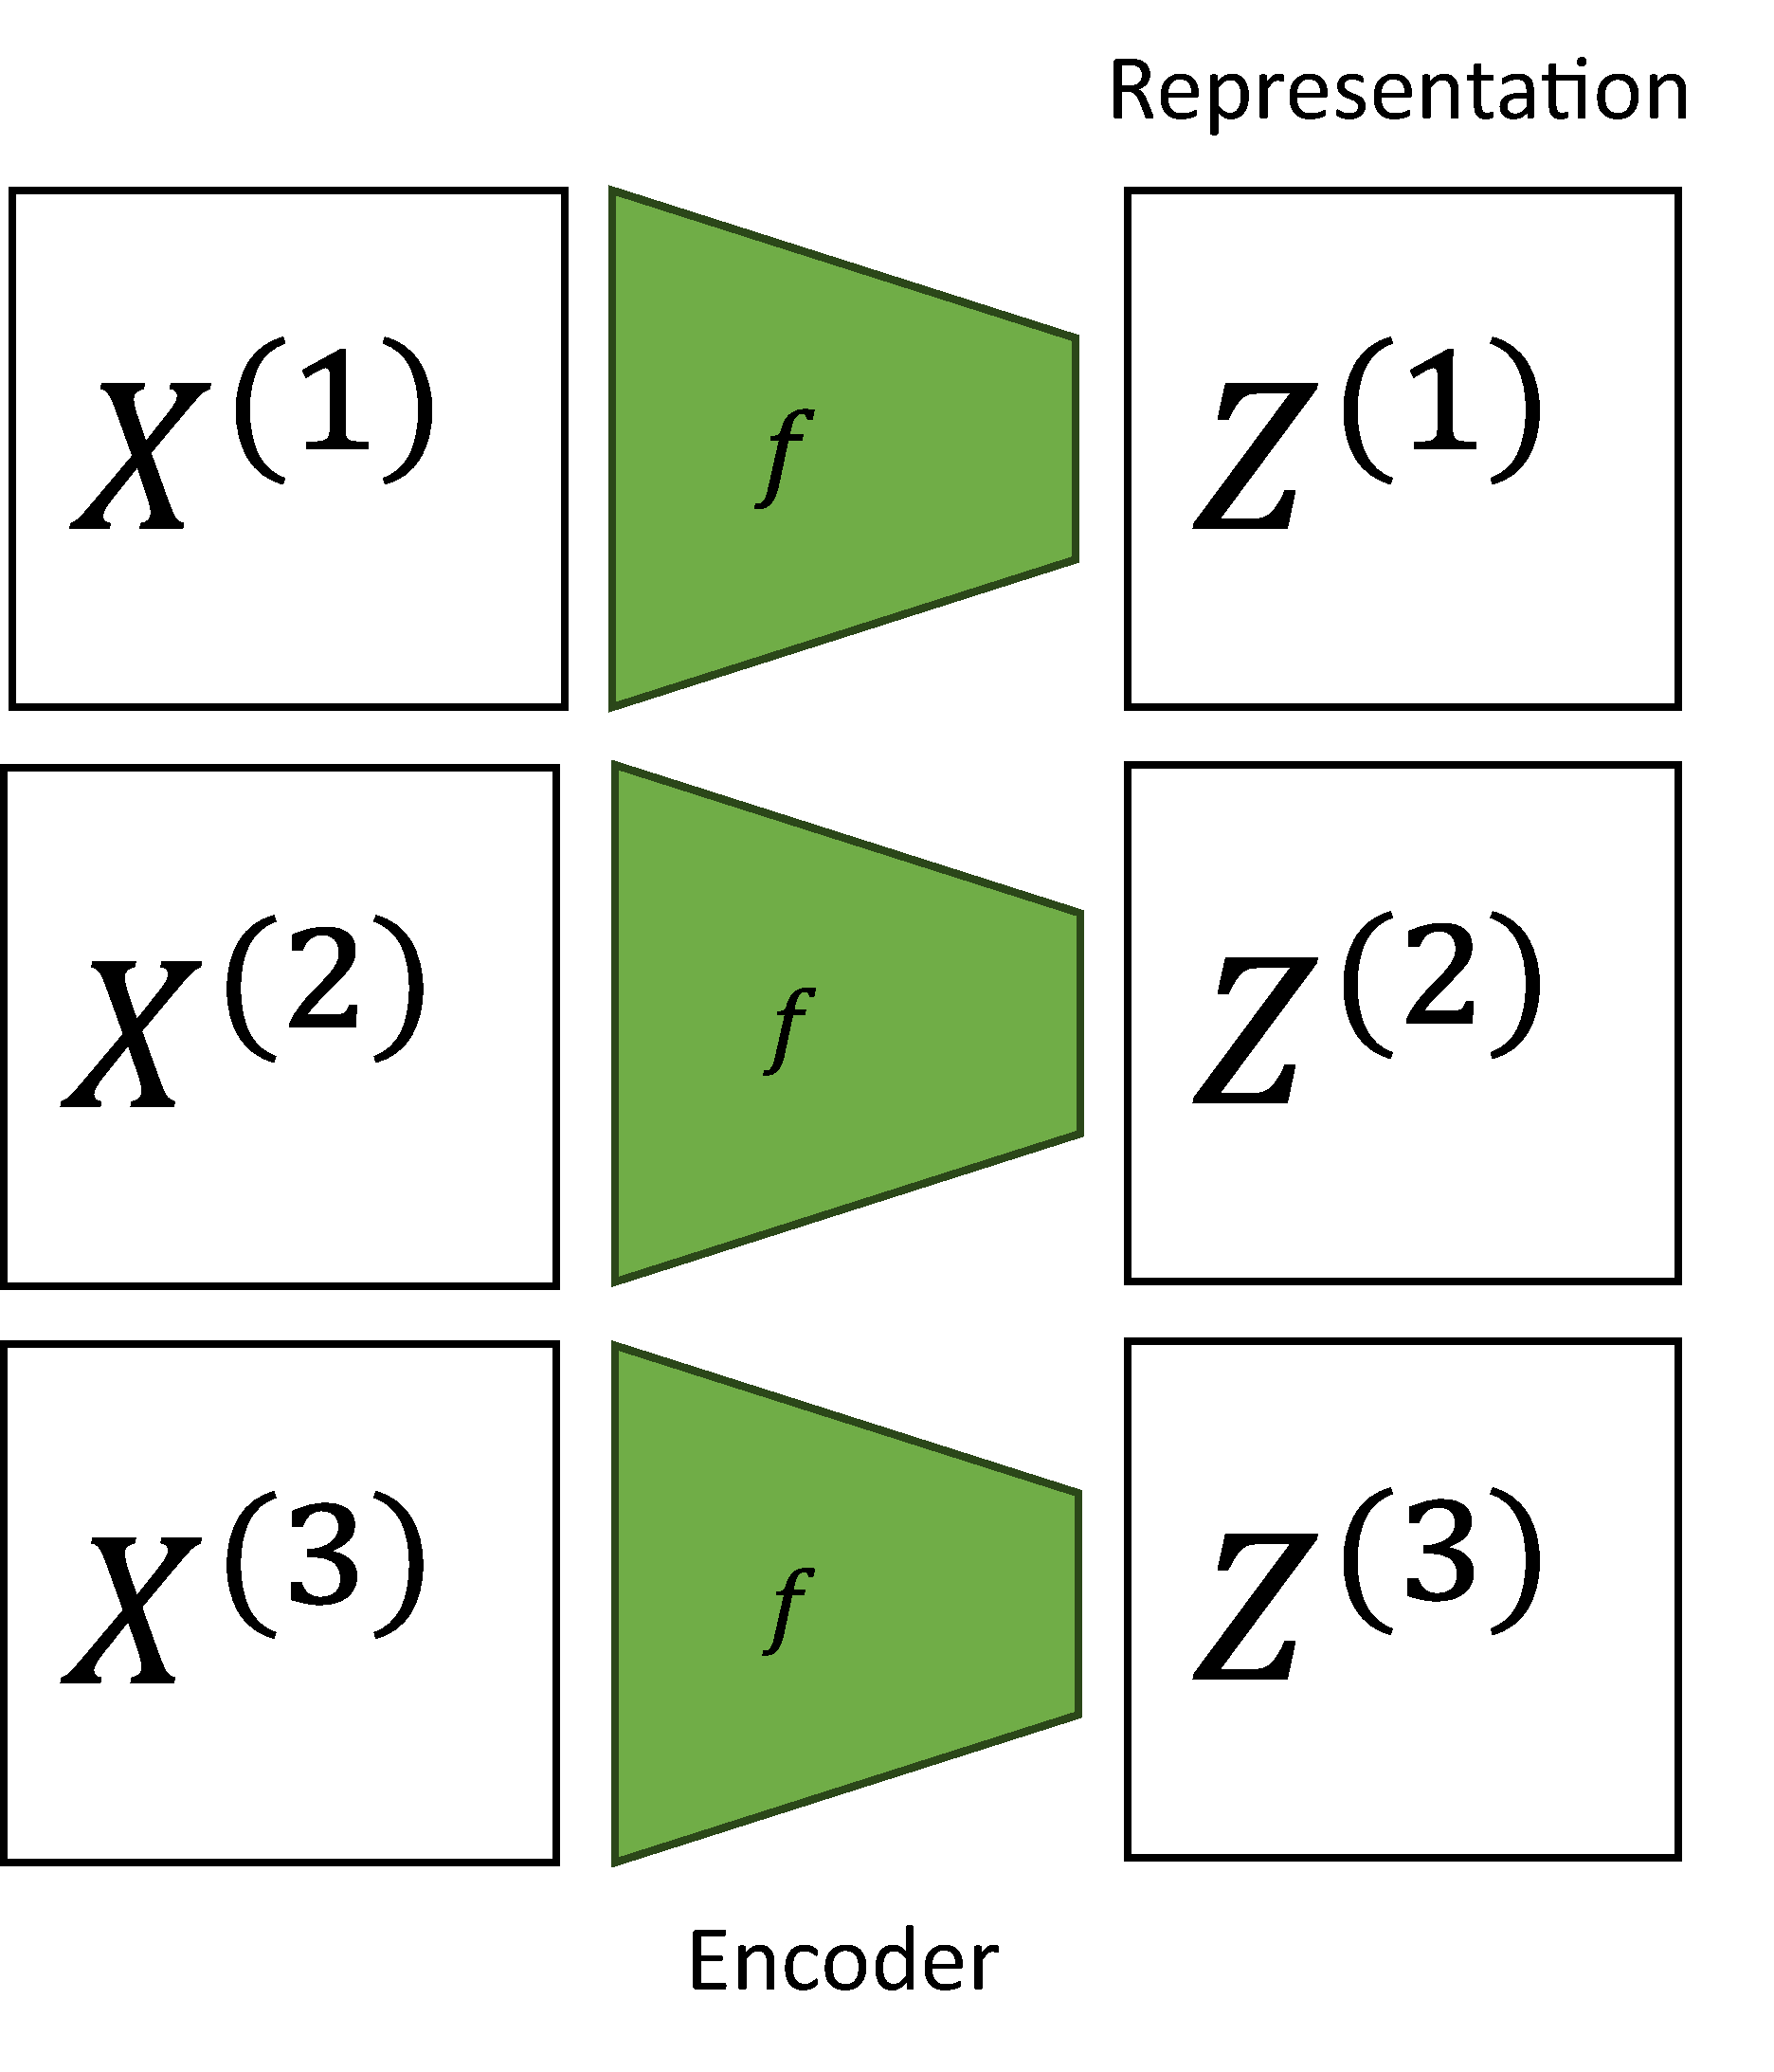
\includegraphics[width=0.4\textwidth]{figures/dcca_schematic}
    \caption{Schematic of the DCCA approach highlighting the nonlinear transformation of data into correlated views.}
    \label{fig:dcca_schematic}
\end{figure}

Figure \ref{fig:dcca_schematic} illustrates the conceptual framework of DCCA, where data from different views are transformed through neural networks to achieve correlated representations.

The full-batch approach of DCCA, formulated by \citet{andrew2013deep}, seeks to maximize the correlation between these different views. The objective, operationalized as a loss function, is defined by the trace of matrix \( T \):
The full-batch approach of DCCA, formulated by \citet{andrew2013deep}, seeks to maximize the correlation between these different views. The objective, operationalized as a loss function, is defined by the trace of matrix \( T \):
\begin{align}
    T &= \left(\text{cov}(Z^{(1)})\right)^{-\frac{1}{2}} Z^{(1)\top} Z^{(2)} \left(\text{cov}(Z^{(2)})\right)^{-\frac{1}{2}} \label{eq:T_definition} \\
    \LRayleigh &= -\Tr(T) \label{eq:loss_function}
\end{align}

This approach, while theoretically sound, faces scalability issues with large datasets. DCCA-STOL, proposed by \citet{wang2015unsupervised}, adapts this objective to large mini-batches but suffers from biased gradients due to the matrix inversions in equation \eqref{eq:T_definition}. This necessitates batch sizes larger than the representation size, limiting its practical application.

Extensions such as DMCCA \citep{somandepalli2019multimodal} and DGCCA \citep{benton2017deep} attempt to mitigate these limitations by forming matrices \( A \) and \( B \) from mini-batch representations for the generalized eigenvalue problem in CCA. However, their loss function, given by
\begin{align}
    \LRayleigh &= -\Tr\left(B^{-\frac{1}{2}} A B^{-\frac{1}{2}}\right),
\end{align}
still encounters similar challenges.

Adaptive whitening methods \citep{wang2015stochastic, chang2018scalable} offer another solution by reducing the bias in the DCCA objective. However, as noted in DCCA-NOI \citep{wang2015unsupervised}, these methods introduce a time constant that complicates analysis and requires extensive tuning.

\begin{align}
    \LNOI &= \|{\tilde{\Sigma}_11}^{-\frac{1}{2}} Z\sps{1}-{\tilde{\Sigma}_{22}}^{-\frac{1}{2}} Z\sps{2}\|^2_F
\end{align}

Where $\tilde{\Sigma}_{11}$ and $\tilde{\Sigma}_{22}$ are estimates of the covariance matrices of $Z\sps{1}$ and $Z\sps{2}$ respectively.
However, the authors of \textbf{DCCA-NOI} highlight that the associated time constant complicates analysis and requires extensive tuning.
These limitations highlight the need for more scalable and efficient nonlinear CCA methods that can handle large datasets without compromising on representation quality or requiring extensive hyperparameter tuning.
\subsection{Self-Supervised Learning}

Self-Supervised Learning (SSL) has become a pivotal approach in deep learning for tasks with scarce labeled data. Central to non-contrastive SSL is creating joint embeddings of augmented images. This method involves generating two different views, \( X_1 \) and \( X_2 \), of the same image \( X \) using augmentation techniques. The goal is to align their representations, \( Z^{(1)} \) and \( Z^{(2)} \), in a shared embedding space, leveraging inherent data patterns to develop rich feature representations without explicit labels. A primary challenge in this approach is preventing the collapse of representations, where models output constant features, ignoring input variability.

\subsubsection{Joint Embedding for SSL and the Role of the Projector}
SSL methods like Barlow Twins and VICReg utilize an encoder-projector model, illustrated in Figure \ref{fig:sslschematic}. Input data is transformed by an encoder \( g \) into representations, which are further processed by a projector \( h \) into higher-dimensional embeddings. These embeddings are key to training, but it's the representations that are critical for downstream tasks. The encoder is typically a neural network tailored to the domain, while the projector is often a simpler multi-layer perceptron.

The essence of joint embedding is that similar inputs, \( X \) and its augmented counterpart \( X' \), should lead to similar embeddings, \( Z \) and \( Z' \). The encoder and projector learn to optimize an objective that measures the closeness of \( Z \) and \( Z' \).

Despite their empirical success, the mechanics behind encoder-projector architectures remain partially elusive. Recent research \cite{ma2023deciphering, jing2021understanding} has started unraveling these complexities, but more understanding is needed. Our approach, grounded in canonical correlation principles, seeks to deepen this understanding and inspire future architectural advancements.

\begin{figure}
    \centering
    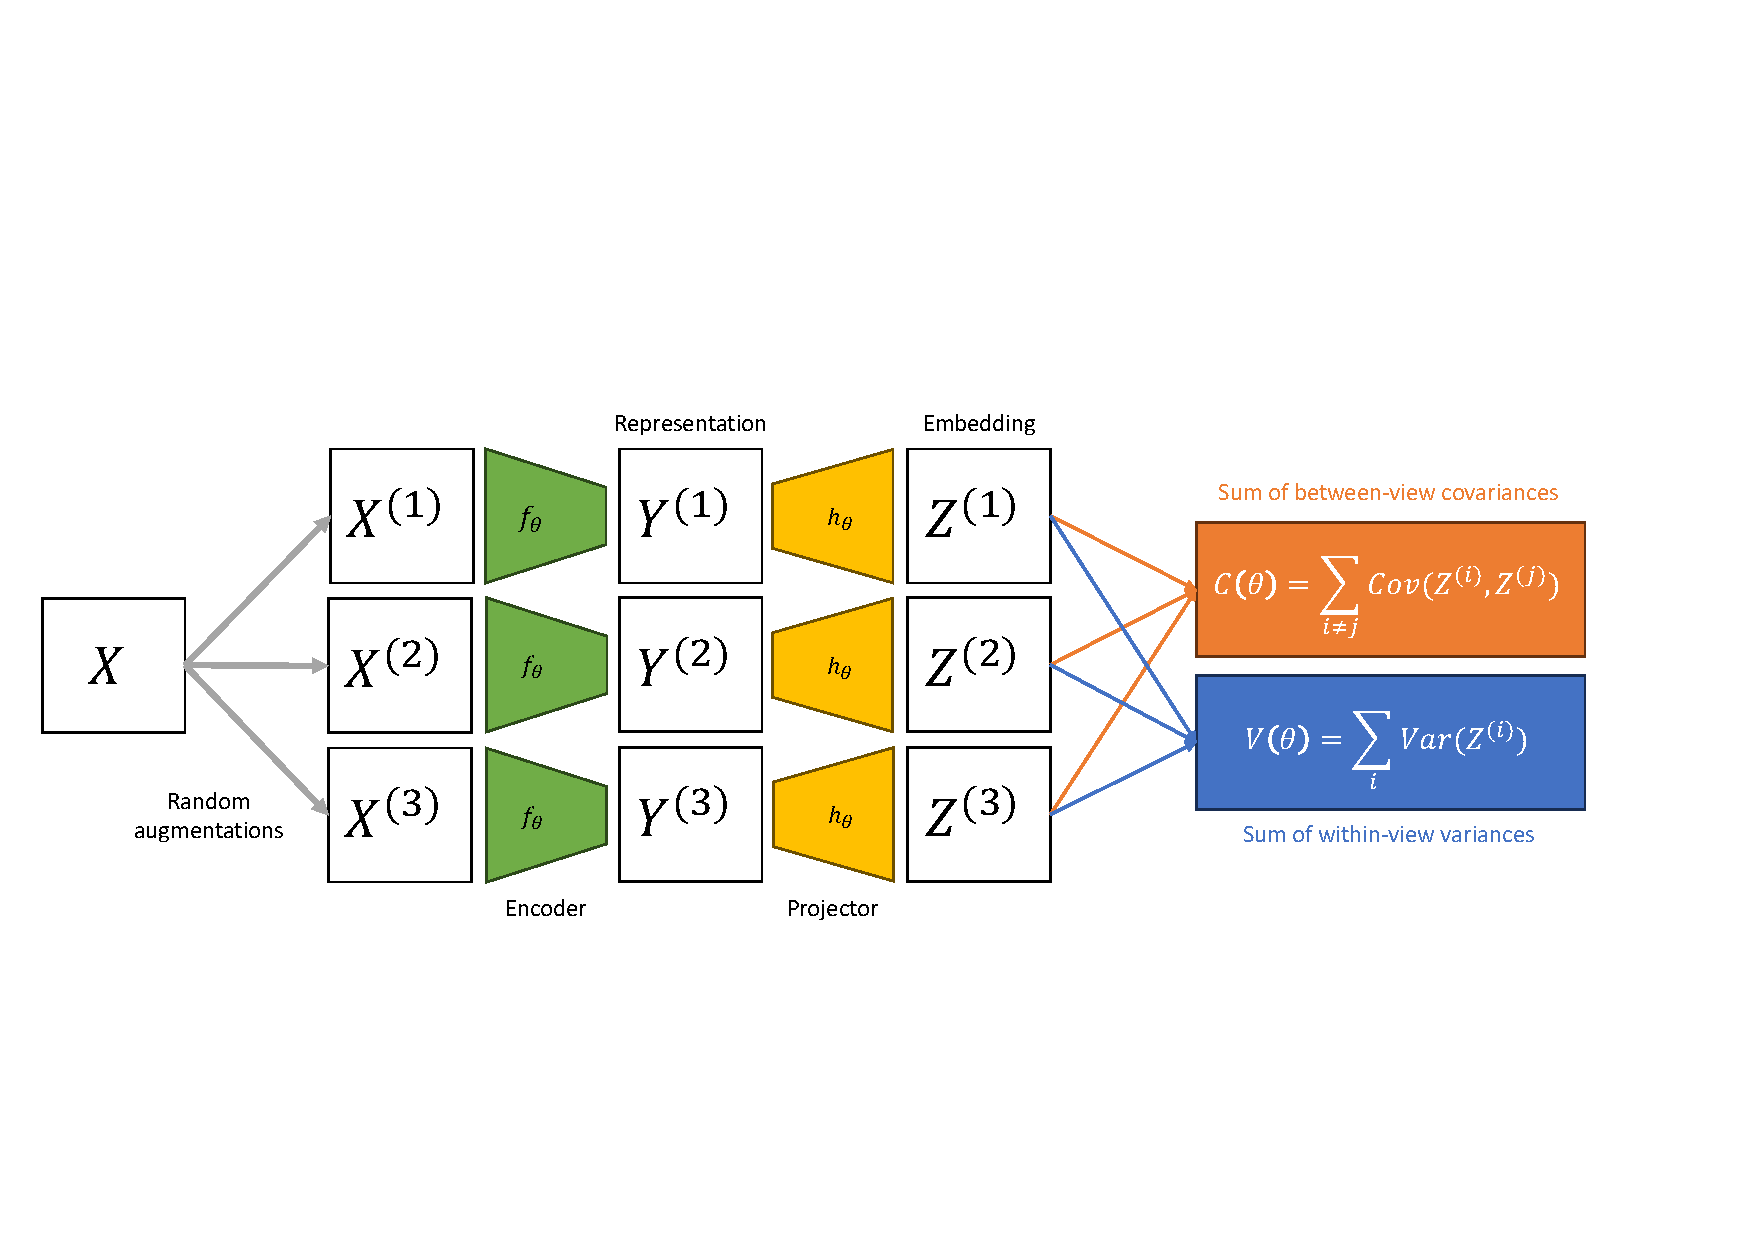
\includegraphics[width=0.8\textwidth]{figures/ssl_schematic}
    \caption{Schematic of the encoder-projector setup in SSL.}
    \label{fig:sslschematic}
\end{figure}

\textbf{Barlow Twins} and \textbf{VICReg}, part of the canonical correlation algorithm family \citep{balestriero2023cookbook}, are pivotal to our study. We first introduce a general form of SSL based on canonical correlation, termed \textbf{CCA-SSL}. Unlike traditional CCA, CCA-SSL employs tied weights for the neural networks, so both views \( Z^{(1)} \) and \( Z^{(2)} \) are functions of the same network \( f_{\theta} \). The general form of CCA-SSL is expressed as:
\begin{align}
    \LCCASSL &= \norm{\MCCA_K\left(Z^{(1)}, Z^{(2)}\right)}_2^2 \label{eq:cca-ssl}
\end{align}
where \( Z^{(i)} = f_{\theta}(X^{(i)}) \) for \( i \in \{1, 2\} \).

In the linear case, CCA-SSL corresponds to a Generalized Eigenvalue Problem (GEP), closely related to both CCA and PCA:
\begin{align}
    \Sigma_{12} + \Sigma_{21} u &= \lambda (\Sigma_{11} + \Sigma_{22}) u \label{eq:gep}
\end{align}

Barlow Twins and VICReg are two influential methods in Self-Supervised Learning (SSL) that build upon canonical correlation principles to generate robust representations from augmented views. Both methods aim to align representations of two augmented views, \( Z^{(1)} \) and \( Z^{(2)} \), while ensuring they are distinct yet correlated.

\textbf{Barlow Twins} employs a redundancy reduction objective, ensuring that representations are both similar for the same augmented views and decorrelated within each view \citep{zbontar2021barlow}. Its loss function is formulated as:
\begin{align}
    \LBT &= \gamma \mathbb{E} \norm{Z^{(1)} - Z^{(2)}}^2 + \beta \sum_{\substack{k,l=1 \\ k \neq l}}^K \Cov(\hat{Z}^{(i)}_k, \hat{Z}^{(i)}_l)^2 \label{eq:bt}
\end{align}
where \( \hat{Z}^{(i)} = \text{BN}(Z^{(i)}) \) represents the batch-normalized versions of the representations. The hyperparameters \( \gamma \) and \( \beta \) control the importance of the similarity and decorrelation terms, respectively.

\textbf{VICReg}, on the other hand, introduces a variance term and forgoes batch normalization, focusing on variance-invariance-covariance regularization \citep{bardes2021vicreg}. The VICReg loss is defined as:
\begin{align}
    \LVR &= \gamma \mathbb{E} \norm{Z^{(1)} - Z^{(2)}}^2 + \sum_{i \in \{1,2\}} \left[\alpha \sum_{k=1}^K \left(1 - \sqrt{\Var(Z^{(i)}_k)}\right)_+ + \beta \sum_{\substack{k,l=1 \\ k \neq l}}^K \Cov(Z^{(i)}_k, Z^{(i)}_l)^2 \right] \label{eq:vicreg}
\end{align}
In VICReg, \( \alpha \), \( \beta \), and \( \gamma \) are tuning parameters that balance the influence of variance, invariance, and covariance regularization.

These methods, by leveraging canonical correlation concepts, serve as foundational baselines in our experiments in SSL.

\section{Methods: Novel Objectives and Algorithms}\label{sec:contributions}

\subsection{Applications to (multi-view) stochastic CCA and PLS, and Deep CCA}

\begin{restatable}{lemma}{recoverDeepCCA}[Objective recovers Deep Multi-view CCA]\label{lem:recover-DeepCCA}
Assume that there is a final linear layer in each neural network $f\sps{i}$.
Then at any local optimum, $\hat{\theta}$, of the population problem, we have
\begin{align*}
    \LEY(\hat{\theta}) = - \norm{\MCCA_K(\hat{Z})}_2^2
\end{align*}
where $\hat{Z} = f_{\hat{\theta}}(X)$.
Therefore, $\hat{\theta}$ is also a local optimum of objectives from \cite{andrew2013deep, somandepalli2019multimodal} as defined in \cref{eq:DMCCA-def}.
\end{restatable}
\begin{proof}[Proof sketch: see \cref{supp:EY-recover-Deep-CCA} for full details.]
    Consider treating the penultimate-layer representations as fixed, and optimising over the weights in the final layer. This is precisely equivalent to optimising the Eckhart-Young loss for linear CCA where the input variables are the penultimate-layer representations. So by \cref{prop:no-spurious}, a local optimum is also a global optimum, and by \cref{prop:EY-charac} the optimal value is the negative sum of squared generalised eigenvalues.
\end{proof}

\subsection{Application to SSL}
We can directly apply Algorithm \ref{alg:general} to SSL.
If we wish to have the same neural network transforming each view, we can simply tie the weights $\theta\sps{1} = \theta\sps{2}$.
When the paired data are generated from applying independent, identically distributed (i.i.d.) augmentations to the same original datum, it is intuitive that tying the weights is a sensible procedure, and perhaps acts as a regulariser.


\section{Experiments}

% Deep CCA Section

\subsection{Deep CCA}\label{sec:experiments-DCCA}
In this experiment, we aim to establish the superiority of our DCCA-EY method over existing Deep Canonical Correlation Analysis (DCCA) approaches as described in \cref{sec:related-work}. We specifically focus on showcasing how DCCA-EY outperforms these methods in terms of correlation capture, convergence speed, and ease of hyperparameter tuning. The experimental setup is aligned with that of \cite{wang2015stochastic}, providing a direct comparison under identical conditions.

As per \citet{wang2015stochastic}, our architecture comprises multilayer perceptrons with two hidden layers of size 800 and an output layer of 50 with ReLU activations. We train these networks for 20 epochs. However, our primary goal is to learn $K=50$ dimensional representations over a range of mini-batch sizes (from 20 to 100) across 50 epochs, demonstrating the robustness and scalability of DCCA-EY even in varying batch conditions.

In this chapter, we employ the Total Correlation Captured (TCC) metric for evaluation. While similar to the PCC metric described in the previous chapter, TCC does not rely on a ground truth for its computation. Instead, it is defined as \( \text{TCC} = \sum_{k=1}^K \rho_k \), where $\rho_k$ are the empirical correlations between the neural network-based representations $Z^{(i)} = f^{(i)}(X^{(i)})$ on a validation set, rather than on the training set as was the case with PCC. This distinction is crucial as TCC evaluates the model's performance in capturing correlations in an unseen dataset, offering a more robust measure of its generalization capability.

\paragraph{Parameters:} For each method, we searched over a hyperparameter grid using \citet{wandb}.

\begin{table}[h!]
    \centering
    \begin{tabular}{|l|l|}
        \hline Parameter           & Values           \\
        \hline minibatch size      & 100, 50, 20      \\
        \hline lr                  & 1e-3, 1e-4, 1e-5 \\
        \hline $\rho$\footnotemark & 0.6, 0.8, 0.9    \\
        \hline epochs              & 50               \\
        \hline
    \end{tabular}
    \footnotetext{$\rho$ is only used for DCCA-NOI}
\end{table}

\paragraph{Observations on SplitMNIST}
For the SplitMNIST dataset, Figure \ref{fig:corr_mnist} shows the comparison of methods across different batch sizes. We observe that DCCA-STOL captures significantly less correlation than the other methods and breaks down when the mini-batch size is smaller than the dimension $K=50$. Figure \ref{fig:lr_mnist} illustrates the learning progress over 50 epochs, where DCCA-NOI, despite performing similarly to DCCA-EY, requires more careful hyperparameter tuning and demonstrates a slower convergence speed.

\paragraph{Observations on XRMB}
On the XRMB dataset, as seen in Figure \ref{fig:corr_xrmb}, similar trends are evident. DCCA-STOL struggles with smaller mini-batch sizes, while DCCA-NOI, though comparable to DCCA-EY in performance, lags in convergence speed, as shown in Figure \ref{fig:lr_xrmb}.

\begin{figure}
    \centering
    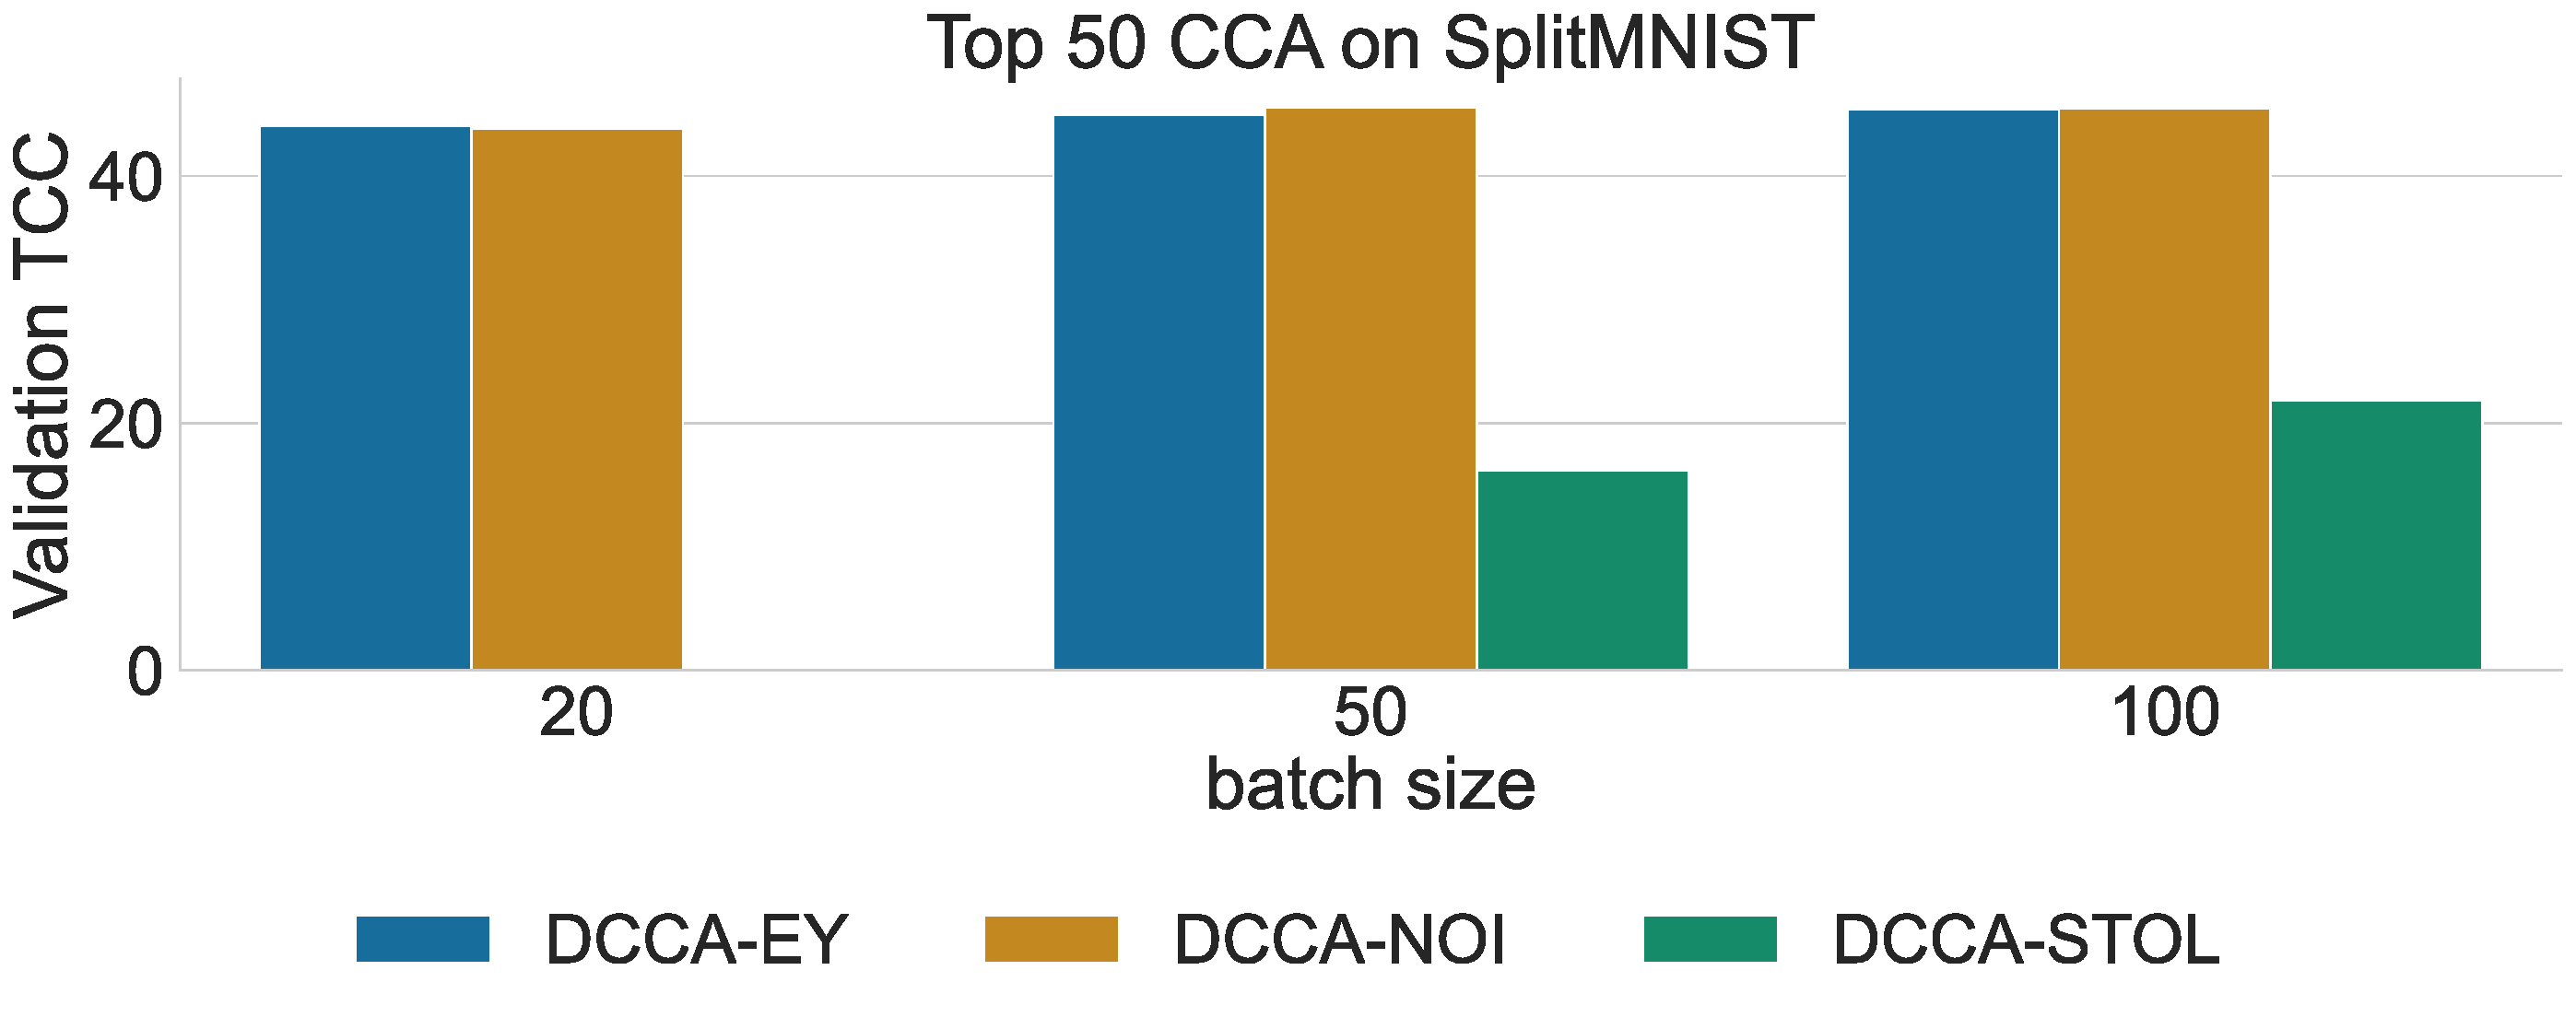
\includegraphics[width=0.7\textwidth]{figures/DCCA/SplitMNIST_models_different_batch_sizes}
    \caption{Deep CCA on SplitMNIST: Comparison of methods across varying batch sizes.}
    \label{fig:corr_mnist}
\end{figure}

\begin{figure}
    \centering
    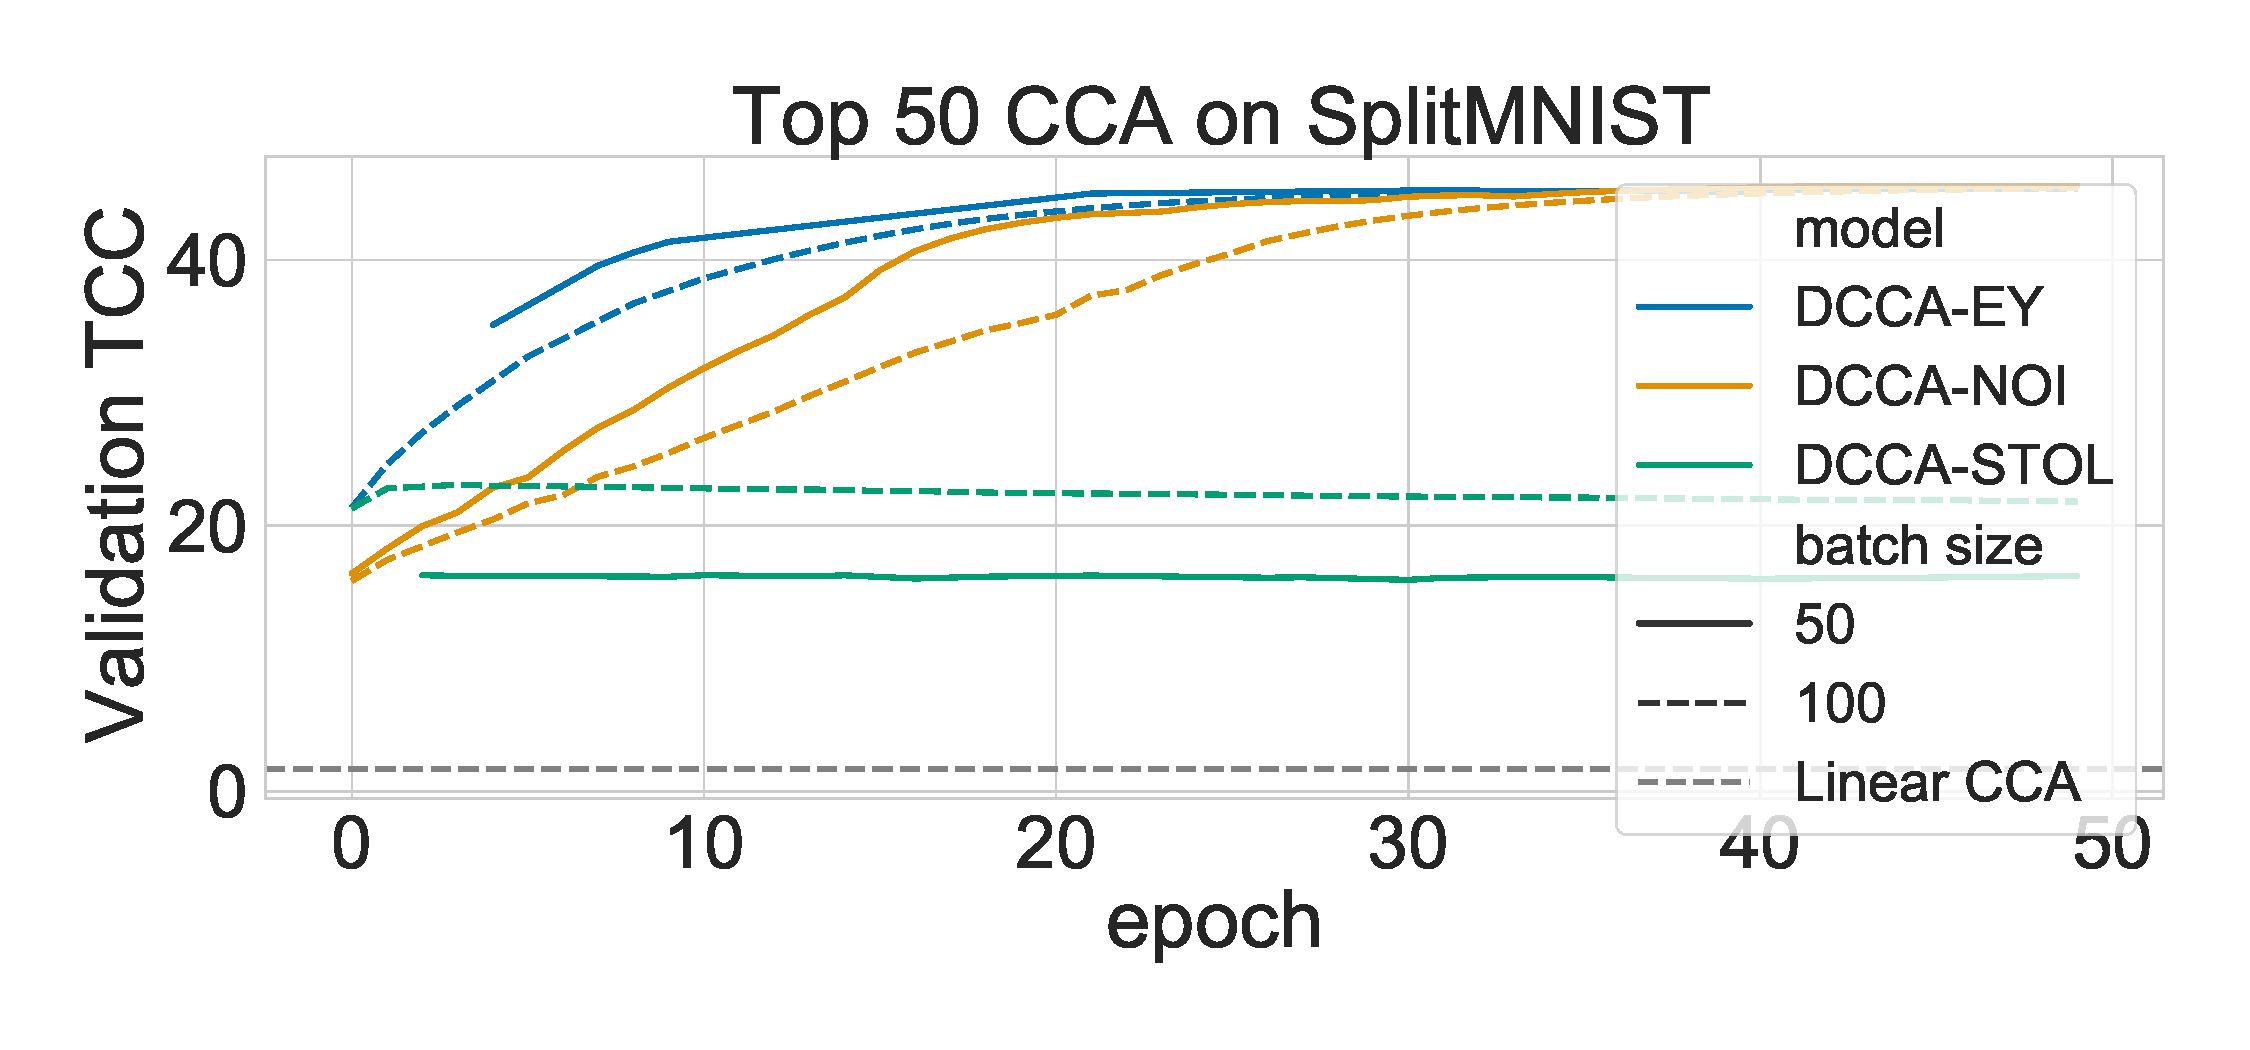
\includegraphics[width=0.7\textwidth]{figures/DCCA/SplitMNIST_allbatchsizes_pcc}
    \caption{Deep CCA on SplitMNIST: Learning progress over 50 epochs.}
    \label{fig:lr_mnist}
\end{figure}

\begin{figure}
    \centering
    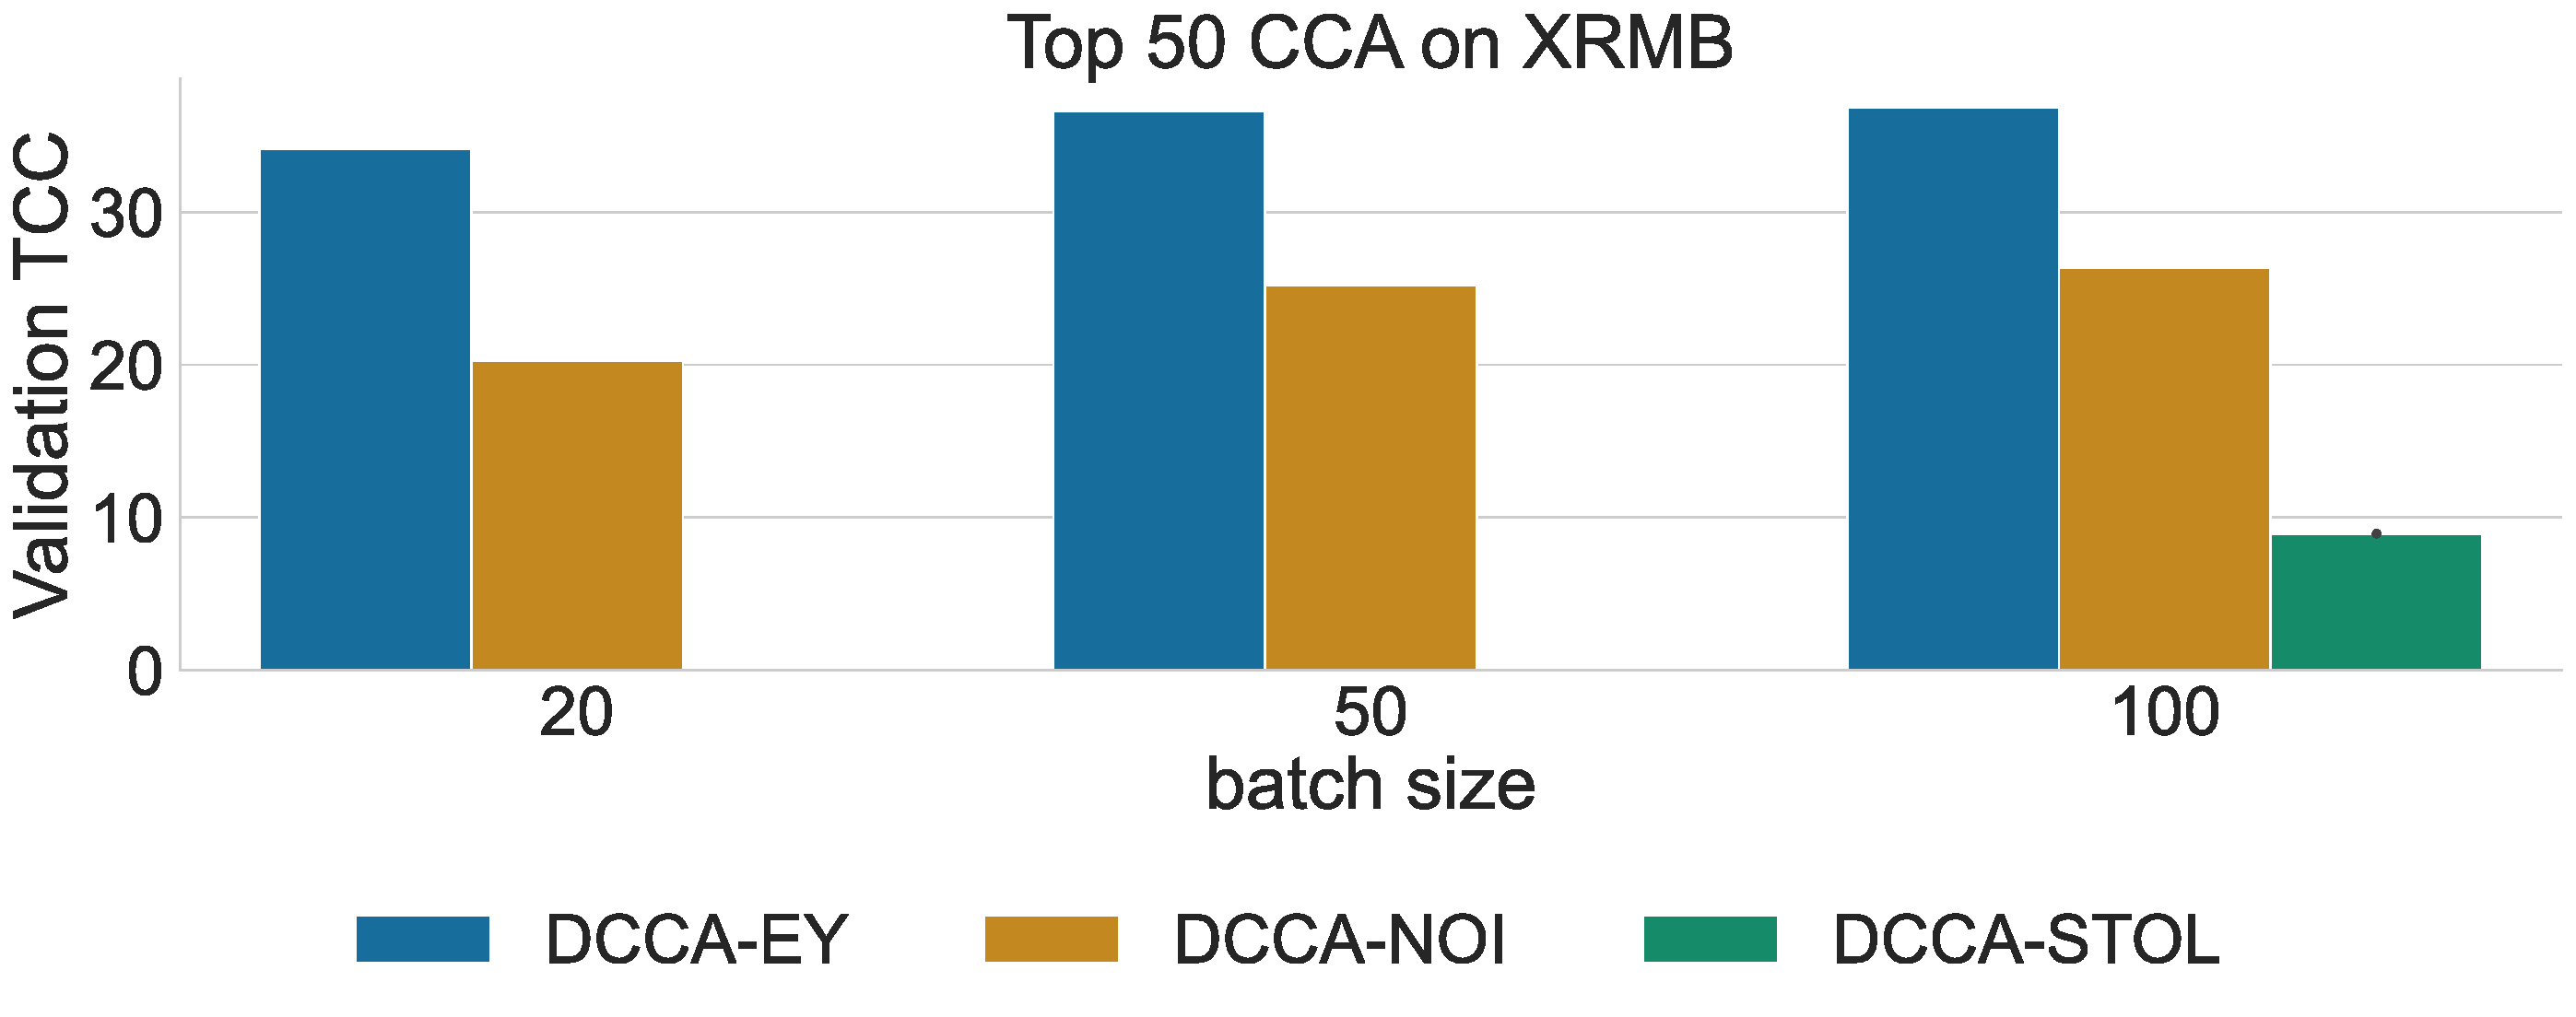
\includegraphics[width=0.7\textwidth]{figures/DCCA/XRMB_models_different_batch_sizes}
    \caption{Deep CCA on XRMB: Comparison of methods across varying batch sizes.}
    \label{fig:corr_xrmb}
\end{figure}

\begin{figure}
    \centering
    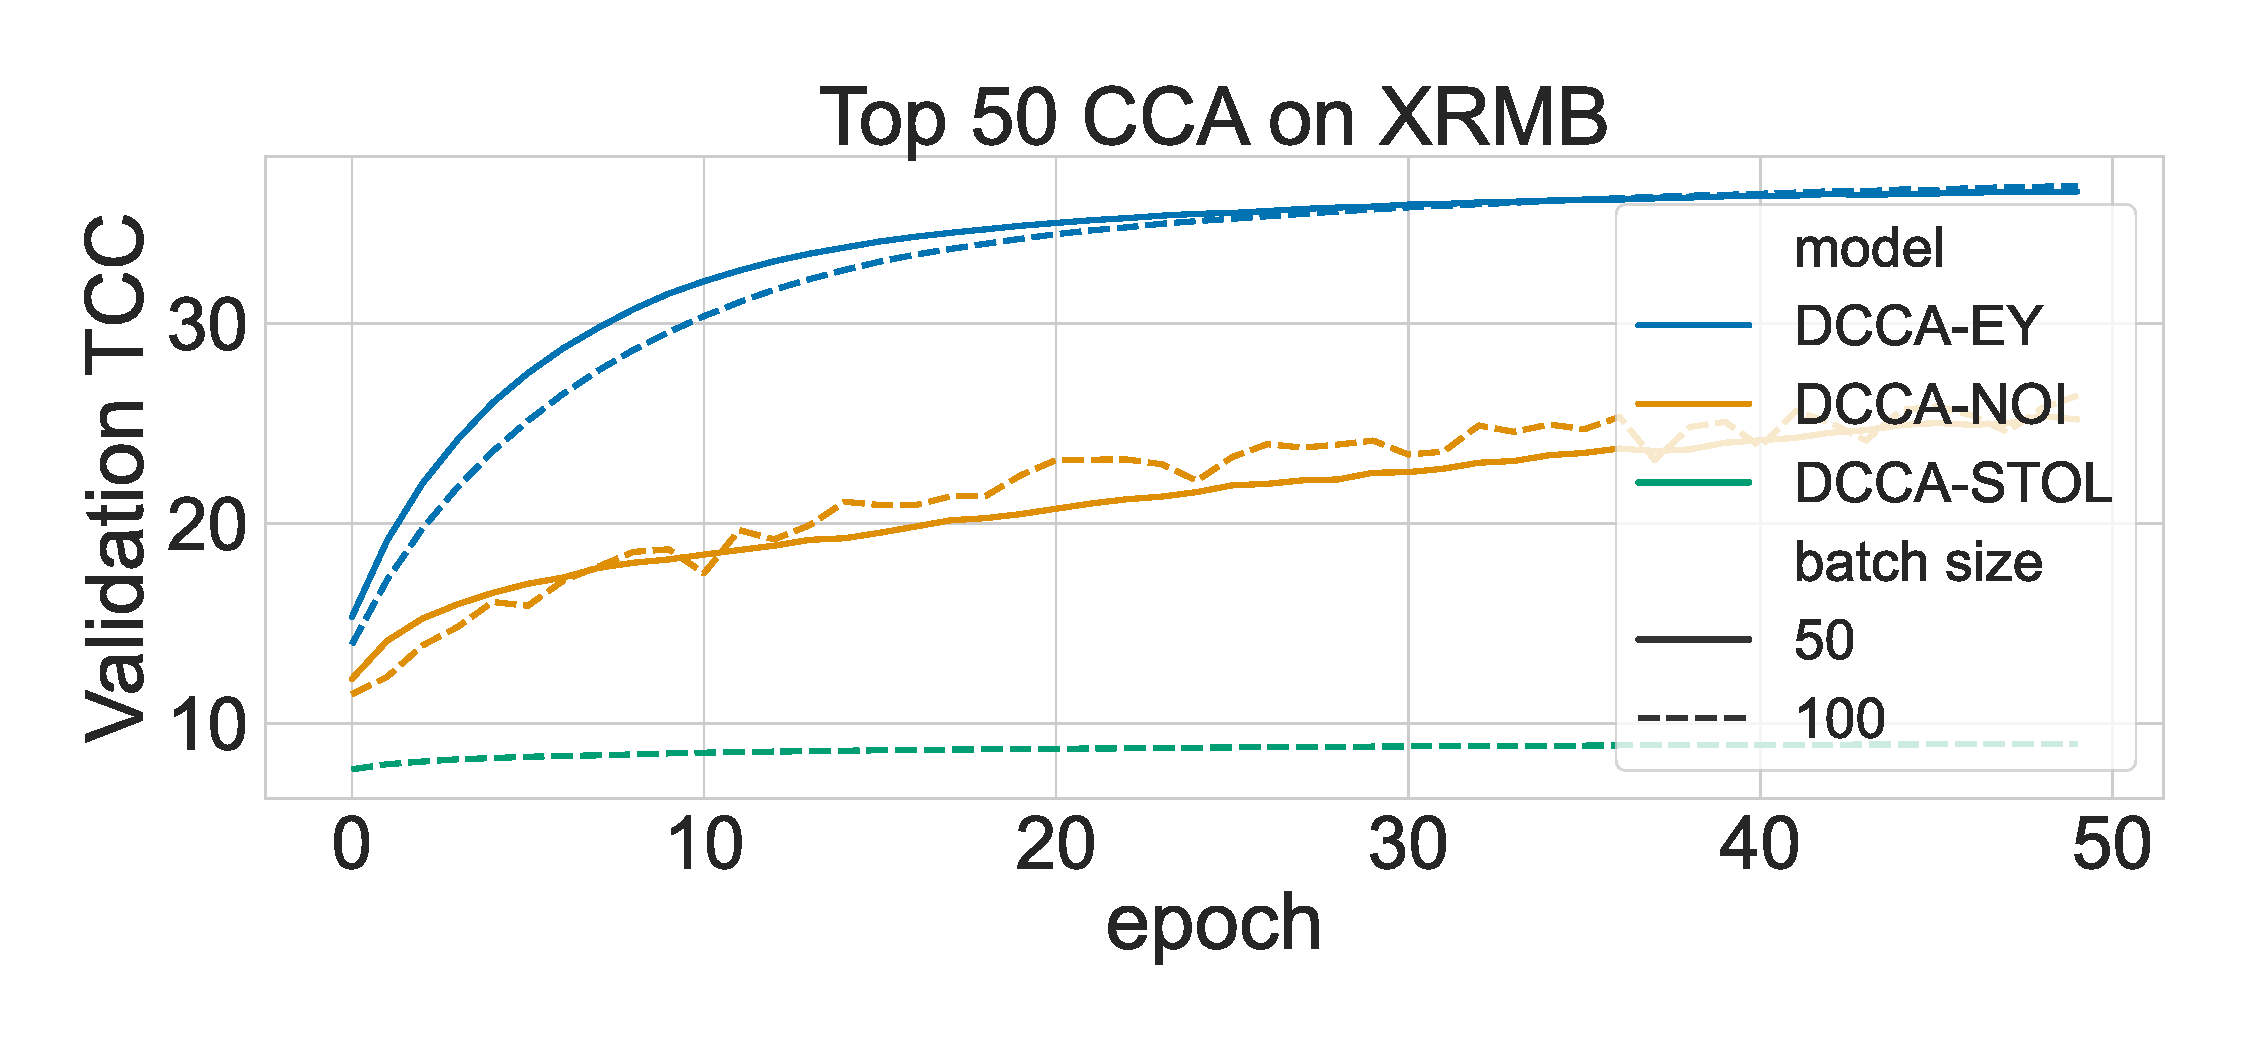
\includegraphics[width=0.7\textwidth]{figures/DCCA/XRMB_allbatchsizes_pcc}
    \caption{Deep CCA on XRMB: Learning progress over 50 epochs.}
    \label{fig:lr_xrmb}
\end{figure}

\subsection{Deep Multiview CCA: Robustness Across Different Batch Sizes}
In our second experiment, our objective is to showcase the adaptability and effectiveness of the DCCA-EY method in the multiview context, particularly in comparison to existing methods such as DMCCA and DGCCA. We choose the mfeat dataset for this purpose, which comprises 2,000 handwritten numeral patterns represented through six distinct feature sets, including Fourier coefficients, profile correlations, Karhunen-Love coefficients, pixel averages in \(2 \times 3\) windows, Zernike moments, and morphological features. These diverse features present an ideal testbed for evaluating the performance of multiview learning methods.
We again learn $K=50$ dimensional representations, but now train for 100 epochs.
We employ a multiview extension of the Total Correlation Captured (TCC) metric, termed Total Multiview Correlation Captured (TMCC). TMCC averages the correlation across views and is defined using the consistent notation from \cref{sec:background-unified} as:
\[
    \text{TMCC} = \sum_{k=1}^{K} \frac{1}{I(I-1)} \sum_{\substack{i,j \leq I \\ i \neq j}} \text{corr}(Z_k^{(i)}, Z_k^{(j)}),
\]
where \( Z_k^{(i)} \) represents the \( k \)-th dimension of the \( i \)-th view's representation. This metric effectively measures the extent to which our method captures correlations between different views in a multidimensional representation space.

\paragraph{Parameters:} For each method, we searched over a hyperparameter grid using \citet{wandb}.

\begin{table}[h!]
    \centering
    \begin{tabular}{|l|l|}
        \hline Parameter      & Values                       \\
        \hline minibatch size & 5,10,20,50,100,200           \\
        \hline components     & 50                           \\
        \hline epochs         & 100                          \\
        \hline lr             & 0.01, 0.001, 0.0001, 0.00001 \\
        \hline
    \end{tabular}
\end{table}

\paragraph{Observations}
Figure~\ref{fig:dmcca_corr} illustrates the comparison of DCCA-EY with DGCCA and DMCCA across different mini-batch sizes, using the validation TMCC metric. DCCA-EY consistently outperforms both DGCCA and DMCCA, showcasing its superior ability to capture validation TMCC. Notably, DMCCA encounters issues when the batch size is smaller than $K=50$, likely due to singular empirical covariances. DGCCA, while not breaking down, significantly underperforms with smaller batch sizes, highlighting limitations in scalability and efficiency for large-scale data applications.

In Figure~\ref{fig:dmcca_lr}, we observe the learning curves for batch sizes 50 and 100. Both DMCCA and DGCCA demonstrate rapid initial learning of significant correlations but reach a plateau relatively quickly. In contrast, DCCA-EY exhibits a consistent improvement over time and notably outperforms the other methods by the end of the training period. This behavior underscores the enhanced learning capability and efficiency of DCCA-EY, especially in the context of large-scale, high-dimensional data.

\begin{figure}
    \centering
    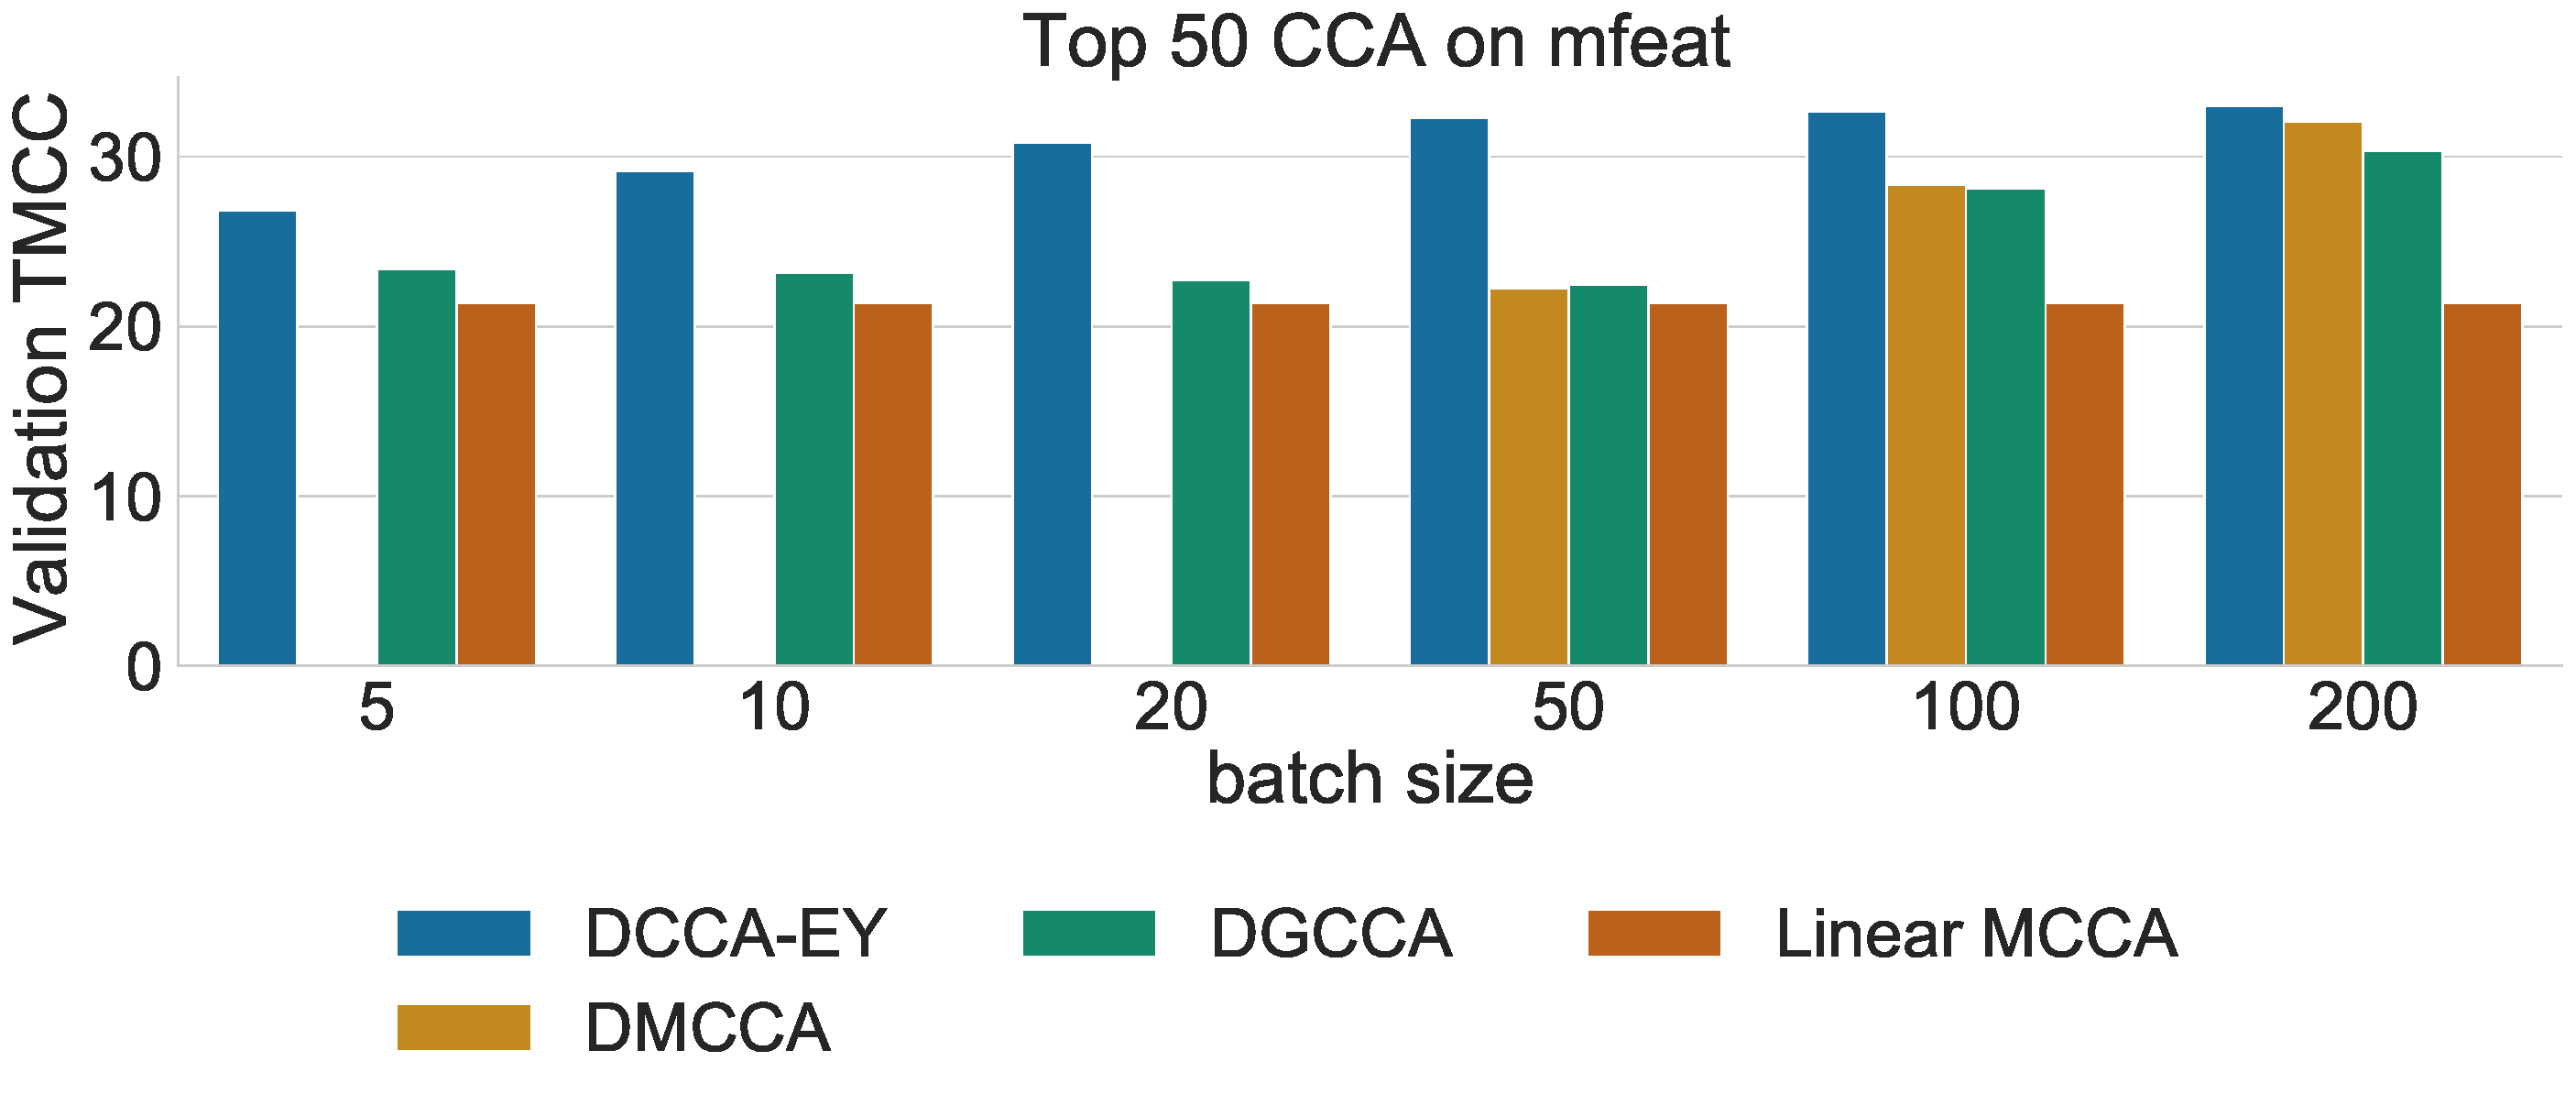
\includegraphics[width=0.49\textwidth]{figures/DMCCA/mfeat_models_different_batch_sizes}
    \caption{Deep Multi-view CCA on mfeat: Comparison across various mini-batch sizes using the Validation TMCC metric.}\label{fig:dmcca_corr}
\end{figure}

\begin{figure}
    \centering
    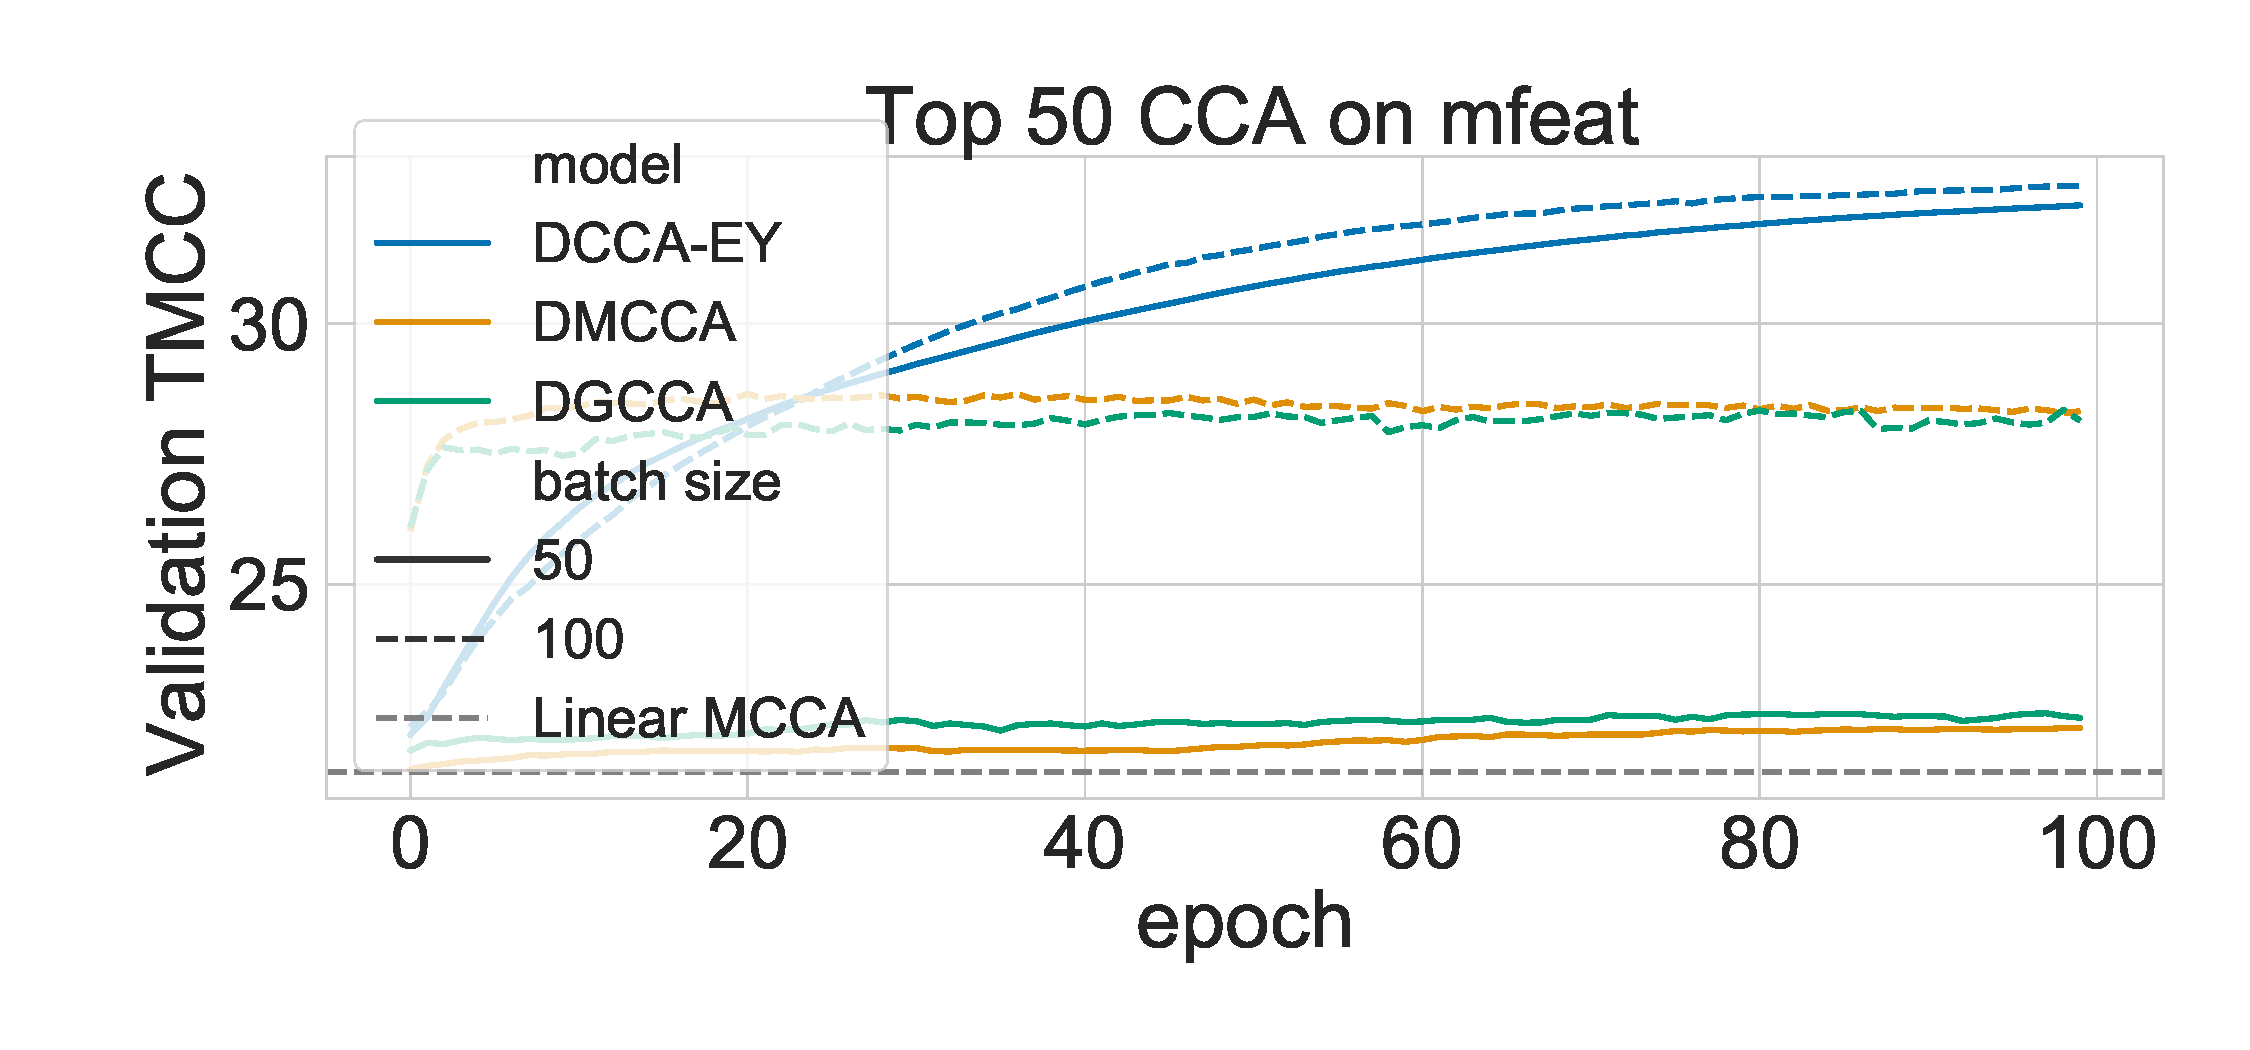
\includegraphics[width=0.49\textwidth]{figures/DMCCA/mfeat_allbatchsizes_pcc}
    \caption{Deep Multi-view CCA on mfeat: Learning progress over 100 epochs for batch sizes 50 and 100.}\label{fig:dmcca_lr}
\end{figure}

\subsection{Self-Supervised Learning with SSL-EY}
Finally, we benchmark our self-supervised learning algorithm, SSL-EY, with Barlow Twins and VICReg on CIFAR-10 and CIFAR-100. Each dataset contains 60,000 labelled images, but these are over 10 classes for CIFAR-10 and 100 classes for CIFAR-100.

We follow a standard experimental design \citep{tong2023emp}. Indeed, we use the sololearn library \citep{da2022solo}, which offers optimized setups particularly tailored for VICReg and Barlow Twins. All methods utilize a ResNet-18 encoder coupled with a bi-layer projector network. Training spans 1,000 epochs with batches of 256 images. For SSL-EY, we use the hyperparameters optimized for Barlow Twins, aiming not to outperform but to showcase the robustness of our method.
We predict labels via a linear probe on the learnt representations and evaluate performance with Top-1 and Top-5 accuracies on the validation set. For more details, refer to the supplementary material \ref{supp:experimental details}.

\paragraph{Observations:} Table \ref{tab:selfsup} shows that SSL-EY is competitive with Barlow Twins and VICReg. This is remarkable because we used out-of-the-box hyperparameters for SSL-EY but used hyperparameters for Barlow Twins and VICReg that had been heavily optimized in previous studies.

\begin{table}
    \centering
    \begin{tabular}{lcccc}
        \hline
        Method          & CIFAR-10 Top-1 & CIFAR-10 Top-5 & CIFAR-100 Top-1 & CIFAR-100 Top-5 \\
        \hline
        Barlow Twins    & \textbf{92.1}  & 99.73          & \textbf{71.38}  & \textbf{92.32}  \\
        VICReg          & 91.68          & 99.66          & 68.56           & 90.76           \\
        \textbf{SSL-EY} & 91.43          & \textbf{99.75} & 67.52           & 90.17           \\
        \hline
    \end{tabular}
    \caption{Performance comparison of SSL methods on CIFAR-10 and CIFAR-100.}
    \label{tab:selfsup}
\end{table}

\paragraph{Model Convergence:} The Learning curves in Figure~\ref{fig:ssl learning curve cifar100 top5} indicate that the performance variation at 1,000 epochs in table \ref{tab:selfsup} mainly results from optimization noise and speed of convergence is similar.

\paragraph{Smaller Projector or None at All:}
One key motivation for projectors is to prevent excessive collapse of meaningful information. Because SSL-EY learns does not suffer from collapse, we had a prior that it may be more robust to projector size, and perhaps even to removing the projector altogether.
For this reason, in another set of experiments, we explored varying the projector's output dimensions from 2048 to 64 and removing the projector completely while holding the encoder output size constant. Figure~\ref{fig: ssl projector dimensions 100} demonstrates that SSL-EY maintains good performance even with a smaller projector, making the representations more efficient than Barlow Twins and VICReg (they contain the same amount of useful information for the classification task in much fewer dimensions). While Figure~\ref{fig: ssl projector dimensions 100} shows the strong performance of Barlow Twins and VICReg at larger projector sizes for this task, we would argue that our objective is more robust to this design choice, potentially offering a more reliable choice for practitioners employing SSL to unfamiliar datasets. At the bottom of Table \ref{tab:selfsup}, we further highlight the efficiency of SSL-EY by showing that our model performs similarly when we have no projector (just using the a 2048 dimensional representation), suggesting that SSL-EY is less reliant on this architecture\footnote{We note that W-MSE, a close relative of our work, also didn't use a projector despite its use being seemingly ubiquitous}. In contrast, we show in appendix \ref{sec:noproj} that Barlow Twins and VICReg's performance drops substantially without the use of a projector.

\paragraph{$\LEY$ is an informative metric:} Figure~\ref{fig:ssl learning curve cifar100 vs corr} offers two key insights. First, it shows that the EY loss, which provides an unbiased estimate of the canonical correlations of the embeddings, is closely related to classification accuracy. This suggests that maximizing canonical correlation is a promising pretext task for self-supervised learning. Second, the figure reveals that even a reduced-dimensionality projector output (64 dimensions) has not reached its full capacity by 1,000 epochs. Specifically, the sum of squared canonical correlations reaches 46, out of a maximum possible value of 64. This indicates that there is still room for further optimization, implying that SSL-EY's representations have not yet saturated their capacity for capturing meaningful information. Lastly, the evolution of the correlation, as measured by $\LEY$, offers a novel way of monitoring model training even without the need for a separate validation task like classification, and could potentially eliminate the requirement for a validation set altogether. This is a particularly interesting direction given recent work on the stepwise eigenvalue behavior of the representations in SSL models \cite{simon2023stepwise}.

\begin{table}[H]
    \centering
    \begin{tabular}{lcccc}
        \hline
        Method          & CIFAR-10 Top-1 & CIFAR-10 Top-5 & CIFAR-100 Top-1 & CIFAR-100 Top-5 \\
        \hline
        Barlow Twins    & \textbf{92.1}  & 99.73          & \textbf{71.38}  & \textbf{92.32}  \\
        VICReg          & 91.68          & 99.66          & 68.56           & 90.76           \\
        \textbf{SSL-EY} & 91.43          & \textbf{99.75} & 67.52           & 90.17           \\
        \hline
        SSL-EY No Proj. & 90.98          & 99.69          & 65.21           & 88.09           \\
        \hline
    \end{tabular}
    \caption{Performance comparison of SSL methods on CIFAR-10 and CIFAR-100.}
    \label{tab:selfsup}
\end{table}

\begin{figure}[H]
    \centering
% 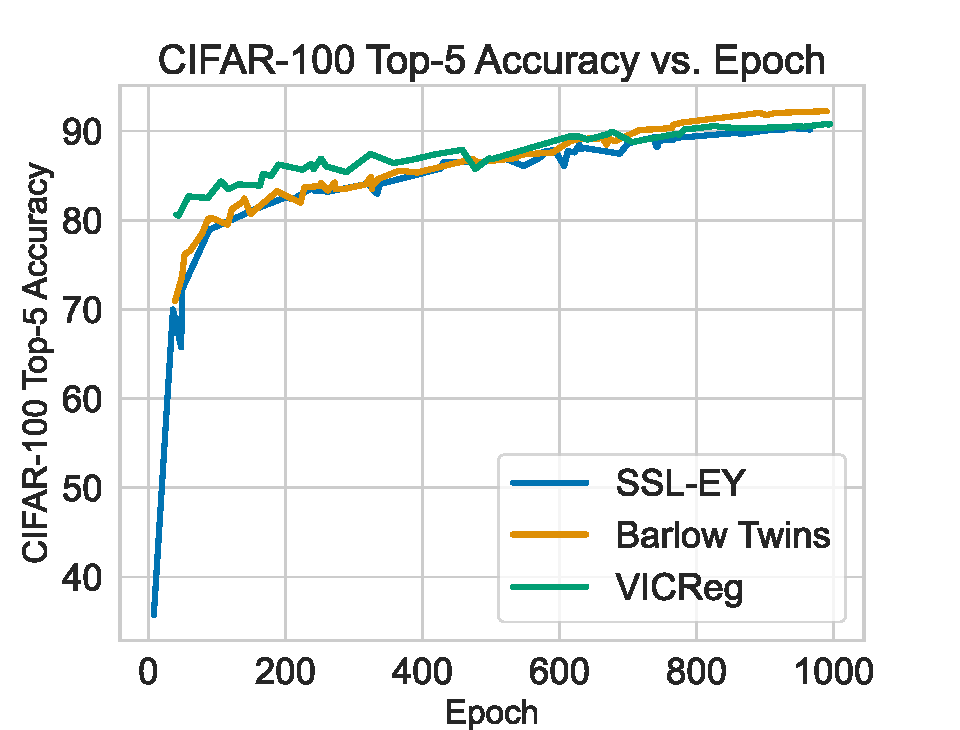
\includegraphics[width=\textwidth]{figures/SSL/cifar100_top5_learning_curve.svg}
    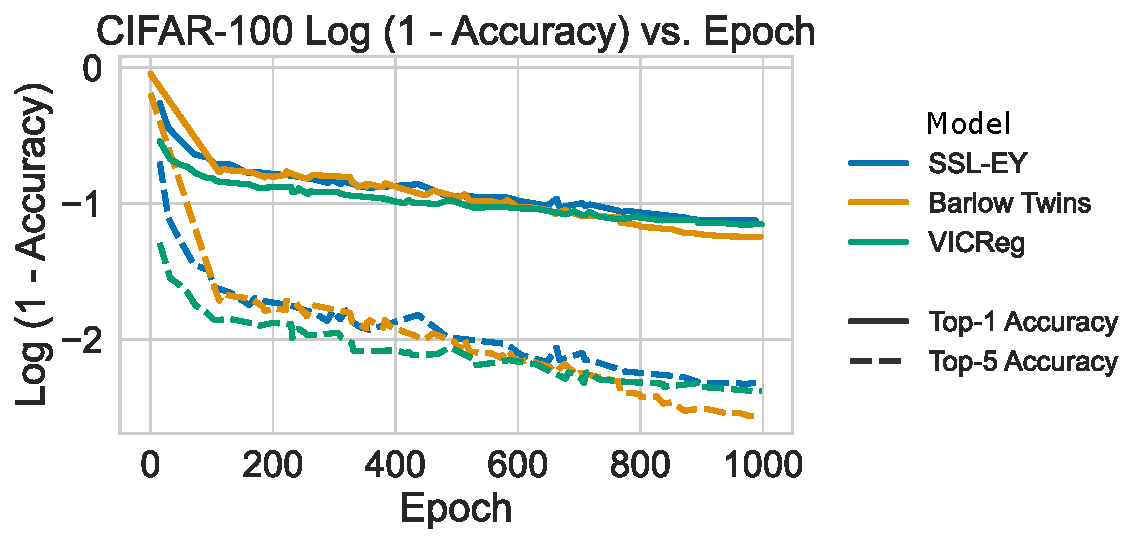
\includegraphics[width=0.57\textwidth]{figures/SSL/cifar100_learning_curve_log_error}
    \caption{\textbf{CIFAR 100: } Learning curves for SSL-EY, Barlow Twins, and VICReg, showing performance across 1,000 epochs.}
    \label{fig:ssl learning curve cifar100 top5}
\end{figure}

\begin{figure}[H]
    \begin{subfigure}[b]{0.47\textwidth}
        \centering
        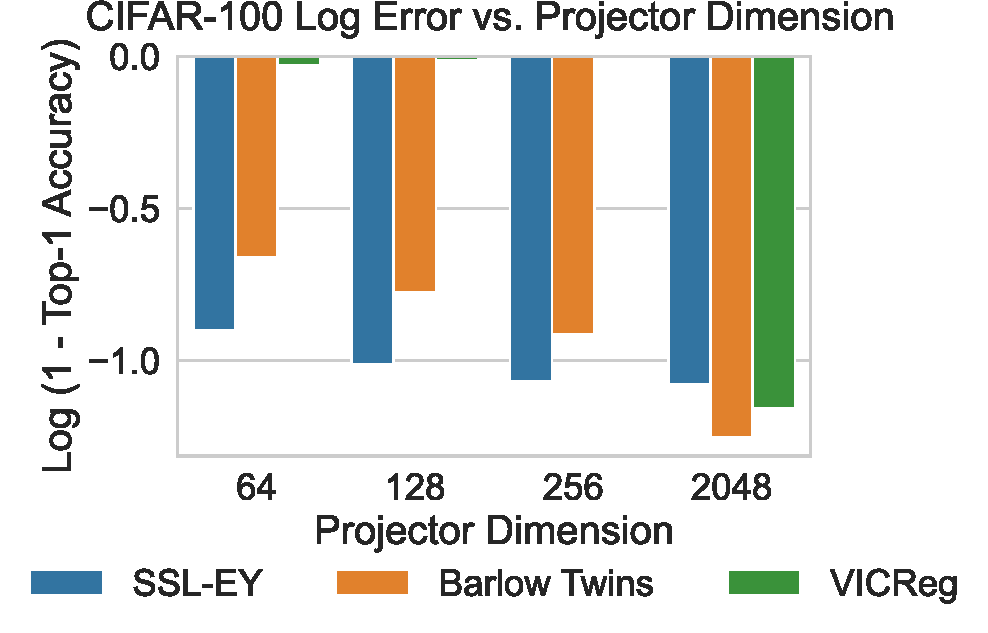
\includegraphics[width=\textwidth]{figures/SSL/cifar100_proj_dim_log_error}
        \caption{}
        \label{fig: ssl projector dimensions 100}
    \end{subfigure}
    \begin{subfigure}[b]{0.47\textwidth}
        \centering
        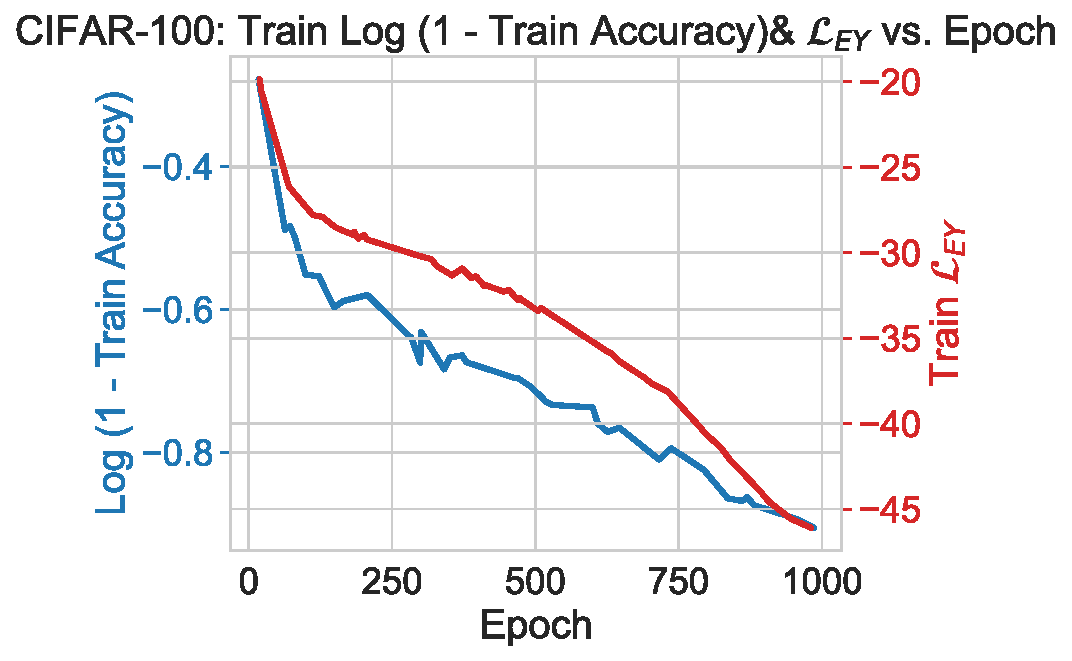
\includegraphics[width=\textwidth]{figures/SSL/cifar100_corr_vs_acc_log_error}
        \caption{}
        \label{fig:ssl learning curve cifar100 vs corr}
    \end{subfigure}
    \caption{\textbf{CIFAR 100: }(a) Performance of SSL-EY with reduced projector size compared to Barlow Twins and VICReg. (b) SSL-EY's learned embeddings indicate untapped representation capacity.}
    \label{fig: ssl projector cifar 100}
\end{figure}


\begin{figure}[H]
    \centering
% 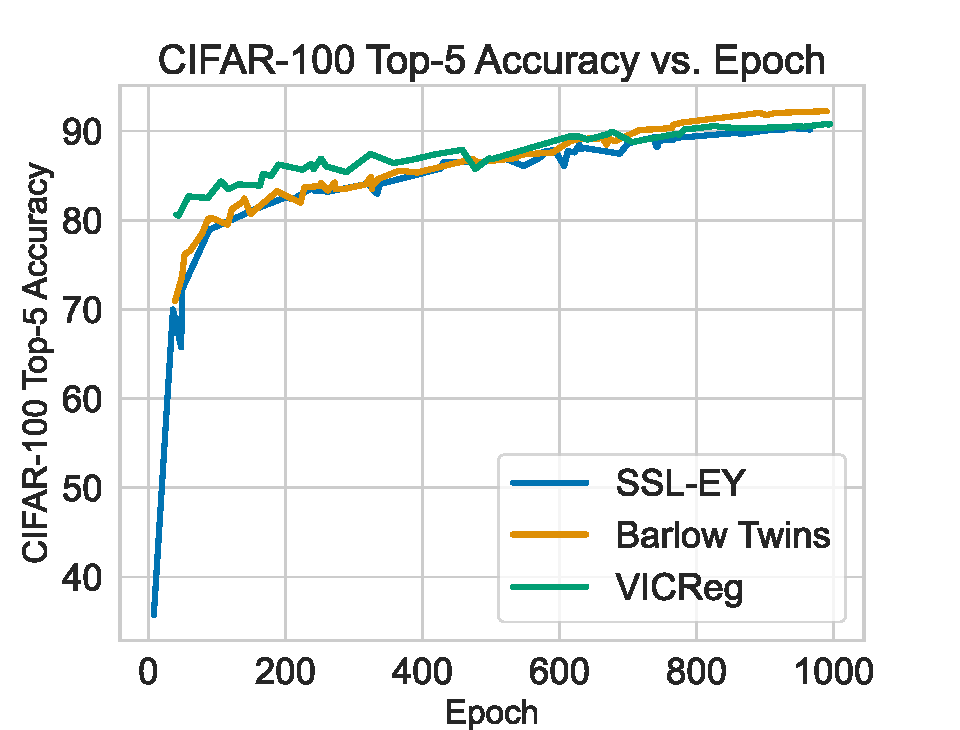
\includegraphics[width=\textwidth]{figures/SSL/cifar100_top5_learning_curve.svg}
    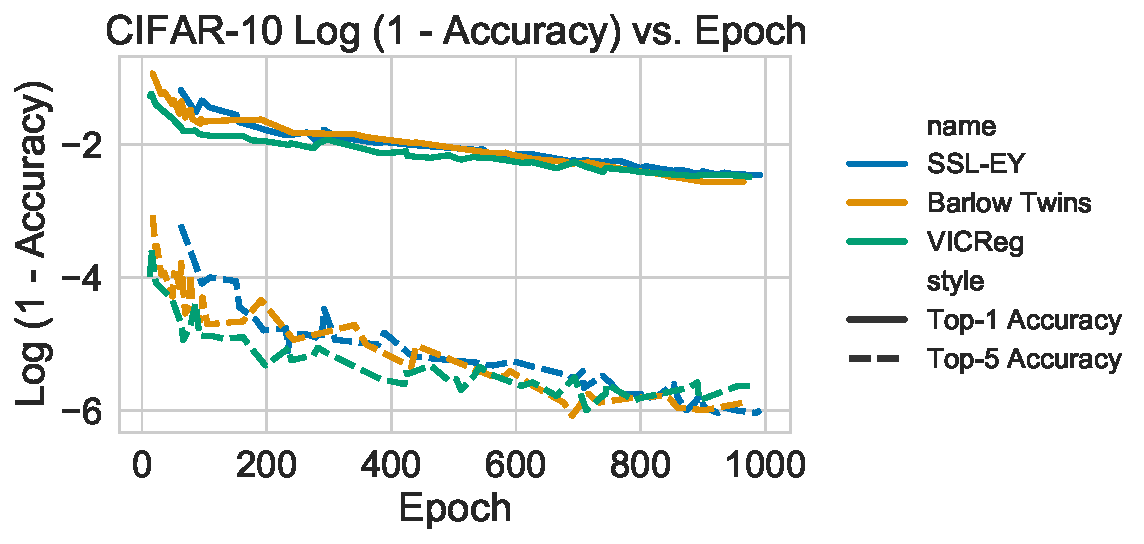
\includegraphics[width=0.57\textwidth]{figures/SSL/cifar10_learning_curve_log_error}
    \caption{\textbf{CIFAR 100: }Learning curves for SSL-EY, Barlow Twins, and VICReg, showing performance across 1,000 epochs.}
    \label{fig:ssl learning curve cifar10 top5}
\end{figure}

\begin{figure}[H]
    \begin{subfigure}[b]{0.47\textwidth}
        \centering
        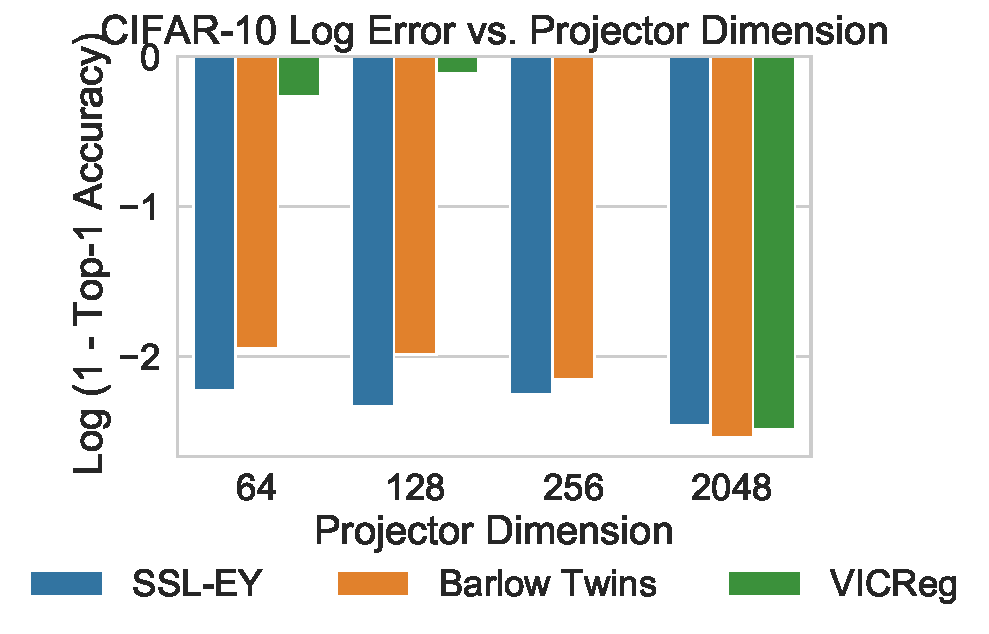
\includegraphics[width=\textwidth]{figures/SSL/cifar10_proj_dim_log_error}
        \caption{}
        \label{fig: ssl projector dimensions 10}
    \end{subfigure}
    \begin{subfigure}[b]{0.47\textwidth}
        \centering
        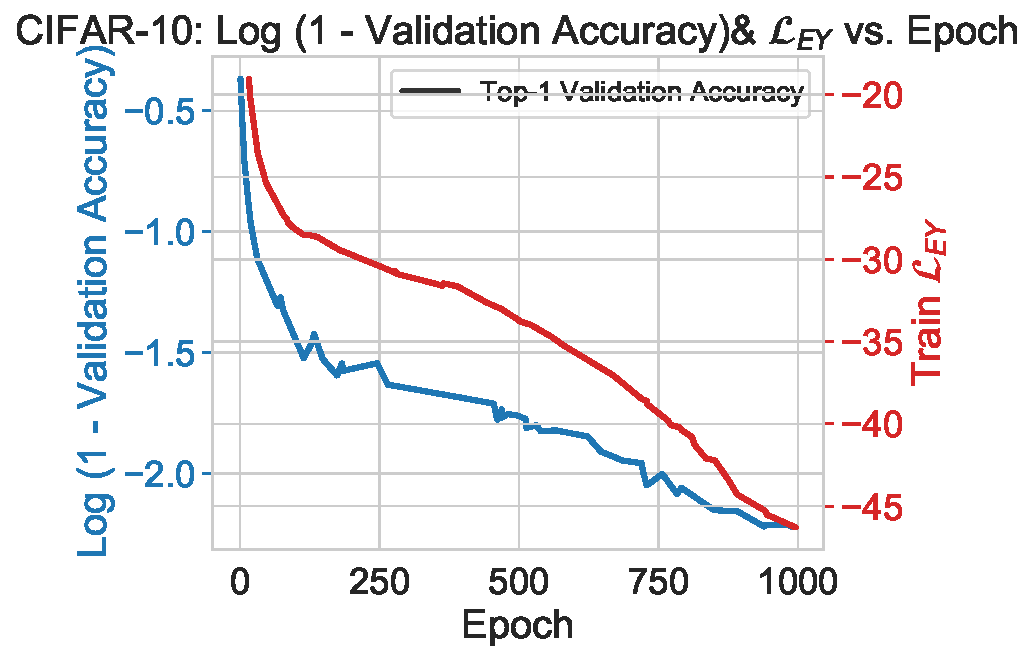
\includegraphics[width=\textwidth]{figures/SSL/cifar10_corr_vs_acc_log_error}
        \caption{}
        \label{fig:ssl learning curve cifar10 vs corr}
    \end{subfigure}
    \caption{\textbf{CIFAR 10: }(a) Performance of SSL-EY with reduced projector size compared to Barlow Twins and VICReg. (b) SSL-EY's learned embeddings indicate untapped representation capacity.}
    \label{fig: ssl projector cifar 10}
\end{figure}

\section{Conclusion}

In this chapter, we extended our work on CCA to the deep learning setting.
We illustrated state-of-the-art performance on the DCCA and DMCCA tasks.
By highlighting links between modern Self-Supervised Learning methods and CCA, we were able to propose a novel self-supervised learning method, SSL-EY, which is competitive with existing methods on CIFAR-10 and CIFAR-100.